% Options for packages loaded elsewhere
\PassOptionsToPackage{unicode}{hyperref}
\PassOptionsToPackage{hyphens}{url}
\PassOptionsToPackage{dvipsnames,svgnames,x11names}{xcolor}
\documentclass[
  12pt,
]{article}
\usepackage{xcolor}
\usepackage[margin=1.0in]{geometry}
\usepackage{amsmath,amssymb}
\setcounter{secnumdepth}{-\maxdimen} % remove section numbering
\usepackage{iftex}
\ifPDFTeX
  \usepackage[T1]{fontenc}
  \usepackage[utf8]{inputenc}
  \usepackage{textcomp} % provide euro and other symbols
\else % if luatex or xetex
  \usepackage{unicode-math} % this also loads fontspec
  \defaultfontfeatures{Scale=MatchLowercase}
  \defaultfontfeatures[\rmfamily]{Ligatures=TeX,Scale=1}
\fi
\usepackage{lmodern}
\ifPDFTeX\else
  % xetex/luatex font selection
    \setmainfont[]{Georgia}
\fi
% Use upquote if available, for straight quotes in verbatim environments
\IfFileExists{upquote.sty}{\usepackage{upquote}}{}
\IfFileExists{microtype.sty}{% use microtype if available
  \usepackage[]{microtype}
  \UseMicrotypeSet[protrusion]{basicmath} % disable protrusion for tt fonts
}{}
\usepackage{setspace}
\makeatletter
\@ifundefined{KOMAClassName}{% if non-KOMA class
  \IfFileExists{parskip.sty}{%
    \usepackage{parskip}
  }{% else
    \setlength{\parindent}{0pt}
    \setlength{\parskip}{6pt plus 2pt minus 1pt}}
}{% if KOMA class
  \KOMAoptions{parskip=half}}
\makeatother
\usepackage{graphicx}
\makeatletter
\newsavebox\pandoc@box
\newcommand*\pandocbounded[1]{% scales image to fit in text height/width
  \sbox\pandoc@box{#1}%
  \Gscale@div\@tempa{\textheight}{\dimexpr\ht\pandoc@box+\dp\pandoc@box\relax}%
  \Gscale@div\@tempb{\linewidth}{\wd\pandoc@box}%
  \ifdim\@tempb\p@<\@tempa\p@\let\@tempa\@tempb\fi% select the smaller of both
  \ifdim\@tempa\p@<\p@\scalebox{\@tempa}{\usebox\pandoc@box}%
  \else\usebox{\pandoc@box}%
  \fi%
}
% Set default figure placement to htbp
\def\fps@figure{htbp}
\makeatother
% definitions for citeproc citations
\NewDocumentCommand\citeproctext{}{}
\NewDocumentCommand\citeproc{mm}{%
  \begingroup\def\citeproctext{#2}\cite{#1}\endgroup}
\makeatletter
 % allow citations to break across lines
 \let\@cite@ofmt\@firstofone
 % avoid brackets around text for \cite:
 \def\@biblabel#1{}
 \def\@cite#1#2{{#1\if@tempswa , #2\fi}}
\makeatother
\newlength{\cslhangindent}
\setlength{\cslhangindent}{1.5em}
\newlength{\csllabelwidth}
\setlength{\csllabelwidth}{3em}
\newenvironment{CSLReferences}[2] % #1 hanging-indent, #2 entry-spacing
 {\begin{list}{}{%
  \setlength{\itemindent}{0pt}
  \setlength{\leftmargin}{0pt}
  \setlength{\parsep}{0pt}
  % turn on hanging indent if param 1 is 1
  \ifodd #1
   \setlength{\leftmargin}{\cslhangindent}
   \setlength{\itemindent}{-1\cslhangindent}
  \fi
  % set entry spacing
  \setlength{\itemsep}{#2\baselineskip}}}
 {\end{list}}
\usepackage{calc}
\newcommand{\CSLBlock}[1]{\hfill\break\parbox[t]{\linewidth}{\strut\ignorespaces#1\strut}}
\newcommand{\CSLLeftMargin}[1]{\parbox[t]{\csllabelwidth}{\strut#1\strut}}
\newcommand{\CSLRightInline}[1]{\parbox[t]{\linewidth - \csllabelwidth}{\strut#1\strut}}
\newcommand{\CSLIndent}[1]{\hspace{\cslhangindent}#1}
\setlength{\emergencystretch}{3em} % prevent overfull lines
\providecommand{\tightlist}{%
  \setlength{\itemsep}{0pt}\setlength{\parskip}{0pt}}
\usepackage{longtable}
\usepackage{graphicx}
\usepackage{booktabs}
\usepackage{textcomp}
\usepackage{xcolor}
\usepackage{colortbl}
\usepackage{geometry}
\usepackage{subcaption}
\usepackage{lineno}
\usepackage{makecell}
\usepackage{pdflscape}
\definecolor{listcomment}{rgb}{0.0,0.5,0.0}
\definecolor{listkeyword}{rgb}{0.0,0.0,0.5}
\definecolor{listnumbers}{gray}{0.65}
\definecolor{listlightgray}{gray}{0.955}
\definecolor{listwhite}{gray}{1.0}
\usepackage{bookmark}
\IfFileExists{xurl.sty}{\usepackage{xurl}}{} % add URL line breaks if available
\urlstyle{same}
\hypersetup{
  colorlinks=true,
  linkcolor={Maroon},
  filecolor={Maroon},
  citecolor={Blue},
  urlcolor={blue},
  pdfcreator={LaTeX via pandoc}}

\author{}
\date{\vspace{-2.5em}}

\begin{document}

\setstretch{1.5}
\linenumbers
\pagenumbering{gobble}

\setstretch{1}

\begin{centering}

$ $

\vspace{6cm}

\LARGE

{\bf Modular strategies for spatial mapping of diverse cell type data of the mouse brain}

\vspace{1.0 cm}

\normalsize

Nicholas J. Tustison$^{1}$,
Min Chen$^{2}$,
Fae N. Kronman$^{3}$,
Jeffrey T. Duda$^{2}$,
Clare Gamlin$^{4}$,
Mia G. Tustison,
Michael Kunst$^{4}$,
Rachel Dalley$^{4}$,
Staci Sorenson$^{4}$,
Quanxin Wang$^{4}$,
Lydia Ng$^{4}$,
Yongsoo Kim$^{3}$, and
James C. Gee$^{2}$

\small

$^{1}$Department of Radiology and Medical Imaging, University of Virginia, Charlottesville, VA \\
$^{2}$Department of Radiology, University of Pennsylvania, Philadelphia, PA \\
$^{3}$Department of Neural and Behavioral Sciences, Penn State University, Hershey, PA \\
$^{4}$Allen Institute for Brain Science, Seattle, WA \\

\end{centering}

\vspace{3.5 cm}

\noindent

\rule{4cm}{0.4pt}

\scriptsize

Corresponding authors:\\

Nicholas J. Tustison, DSc\\
Department of Radiology and Medical Imaging\\
University of Virginia\\
\href{mailto:ntustison@virginia.edu}{\nolinkurl{ntustison@virginia.edu}}\\

James C. Gee, PhD\\
Department of Radiology\\
University of Pennsylvania\\
\href{mailto:gee@upenn.edu}{\nolinkurl{gee@upenn.edu}}

\normalsize

\newpage

\setstretch{1.5}

\section*{Abstract}\label{abstract}
\addcontentsline{toc}{section}{Abstract}

Large-scale, international collaborative efforts by members of the BRAIN
Initiative Cell Census Network (BICCN) consortium are aggregating the
most comprehensive reference database to date for diverse cell type
profiling of the mouse brain, which encompasses over 40 different
multi-modal profiling techniques from more than 30 research groups. One
central challenge for this integrative effort has been the need to map
these unique datasets into common reference spaces such that the
spatial, structural, and functional information from different cell
types can be jointly analyzed. However, significant variation in the
acquisition, tissue processing, and imaging techniques across data types
makes mapping such diverse data a multifarious problem. Different data
types exhibit unique tissue distortion and signal characteristics that
precludes a single mapping strategy from being generally applicable
across all cell type data. Tailored mapping approaches are often needed
to address the unique barriers present in each modality. This work
highlights modular atlas mapping strategies developed across separate
BICCN studies using the Advanced Normalization Tools Ecosystem (ANTsX)
to map spatial transcriptomic (MERFISH) and high-resolution morphology
(fMOST) mouse brain data into the Allen Common Coordinate Framework
(AllenCCFv3), and developmental (MRI and LSFM) data into the
Developmental Common Coordinate Framework (DevCCF). We discuss common
mapping strategies that can be shared across modalities and driven by
specific challenges from each data type. These mapping strategies
include novel open-source contributions that are made publicly available
through ANTSX. These include 1) a velocity flow-based approach for
continuously mapping developmental trajectories such as that
characterizing the DevCCF and 2) an automated framework for determining
structural morphology solely through the leveraging of publicly
resources. Finally, we provide general guidance to aid investigators to
tailor these strategies to address unique data challenges without the
need to develop additional specialized software.

\clearpage

\section{Introduction}\label{introduction}

Over the past decade there have been significant advancements in
mesoscopic single-cell analysis of the mouse brain. It is now possible
to track single neurons in mouse brains\textsuperscript{1}, observe
whole brain developmental changes on a cellular
level\textsuperscript{2}, associate brain regions and tissues with their
genetic composition\textsuperscript{3}, and locally characterize neural
connectivity\textsuperscript{4}. Much of these scientific achievements
have been made possible due to breakthroughs in high resolution cell
profiling and imaging techniques that permit submicron, multi-modal, 3-D
characterizations of whole mouse brains. Among these include advanced
techniques such as micro-optical sectioning
tomography\textsuperscript{6}, tissue clearing\textsuperscript{1,7},
spatial transcriptomics\textsuperscript{9}, and single-cell genomic
profiling\textsuperscript{10}, which have greatly expanded the
resolution and specificity of single-cell measurements in the brain.

Recent efforts by the National Institutes of Health's Brain Research
Through Advancing Innovative Neurotechnologies (BRAIN) Initiative has
pushed for large-scale, international collaborative efforts to utilize
these advanced single-cell techniques to create a comprehensive
reference database for high-resolution transcriptomic, epigenomic,
structural and imaging data of the mouse brain. This consortium of
laboratories and data centers, known as the BRAIN Initiative Cell Census
Network (BICCN), has archived datasets encompassing over 40 different
multi-modal profiling techniques from more than 30 research groups, each
providing unique characterizations of distinct cell types in the
brain\textsuperscript{11}. Several of these modalities have been further
developed into reference atlases to facilitate spatial alignment of
individual brains and different data types into a common coordinate
framework (CCF), thus allowing diverse single-cell information to be
analyzed in an integrated manner. The most notable of these atlases is
the Allen Mouse Brain Common Coordinate Framework
(AllenCCFv3)\textsuperscript{12}, which serves as a primary target
coordinate space for much of the work associated with the BICCN. Other
atlases include modality-specific atlases\textsuperscript{13--15}, and
spatiotemporal atlases\textsuperscript{16,17} for the developing mouse
brain.

\subsection{Mouse brain mapping}\label{mouse-brain-mapping}

The cross-modality associations that can be learned from mapping
different cell type data into a CCF is critical for improving our
understanding of the complex relationships between cellular structure,
morphology, and genetics in the brain. However, finding an accurate
mapping between each individual mouse brain and a CCF is a challenging
and heterogeneous task. There is significant variance in the imaging
protocols across different cell type data as well as different tissue
processing and imaging methods which can potentially introduce tissue
distortion and signal differences\textsuperscript{18,19}. Certain
modalities can have poor intensity correspondence with the CCF,
negatively impacting image alignment accuracy. Studies targeting
specific regions or cell types can lead to missing anatomical
correspondences. Other considerations include artifacts such as tissue
distortion, holes, bubbles, folding, tears, and missing sections in the
data that often require manual correction\textsuperscript{20--23}. Given
the diversity of these challenges, it is unlikely any single mapping
approach can be generally applicable across all cell type data. Diverse,
and often specialized, strategies are needed to address the unique
barriers present for mapping each modality.

Existing solutions to address mapping cell type data into the AllenCCFv3
falls broadly into three main categories. The first consists of
integrated processing platforms that directly provide mapped data to the
users. These include the Allen Brain Cell Atlas\textsuperscript{24} for
the Allen Reference Atlas (ARA) and associated data, the Brain
Architecture Portal\textsuperscript{25} for combined ex vivo radiology
and histology data, OpenBrainMap\textsuperscript{26} for connectivity
data, and the Image and Multi-Morphology Pipeline\textsuperscript{27}
for high resolution morphology data. These platforms provide users
online access to pre-processed, multi-modal cell type data that are
already mapped to the AllenCCFv3. The platforms are designed such that
the data is interactively manipulated by users through integrated
visualization software that allow users to spatially manipulate and
explore each dataset within the mapped space. While highly convenient
for investigators who are interested in studying the specific modalities
provided by these platforms, these systems can be limited in
flexibility, general applicability, and public availability. As a
result, investigators often find it difficult to apply the same mapping
solutions to their own data.

The second category comprises specialized approaches specifically
designed for mapping one or more modalities into a CCF. These approaches
use combinations of specialized manual and automated processes that
address specific challenges in each modality. Examples include
approaches for mapping histology\textsuperscript{28--30}, magnetic
resonance imaging (MRI)\textsuperscript{37}, micro-computed tomography
(microCT)\textsuperscript{35,37}, light-sheet fluorescence microscopy
(LSFM)\textsuperscript{34,36--39}, fluorescence micro-optical sectioning
tomography (fMOST)\textsuperscript{15,40} and transcriptomic
data\textsuperscript{41--43}. As specialized approaches, these
techniques tend to boast higher mapping accuracy, robustness, and ease
of use. Conversely, their specialized designs often rely on base
assumptions regarding the data type that can make them rigid and
difficult to adapt for new modalities or unexpected artifacts and
distortions in the data. Adapting these specialize software tools to use
with new data can require significant development, validation time, and
engineering expertise that may not be readily available for all
investigators.

The last category consists of modular mapping approaches constructed
using general image analysis toolkits, which are software packages that
include modular image processing, segmentation and registration tools
that have been previously developed, and validated for multiple
application areas. Examples of such toolkits include
elastix\textsuperscript{44}, Slicer3D\textsuperscript{45},
ANTsX\textsuperscript{46}, and several others which have all been
applied towards mouse brain spatial mapping (e.g.,\textsuperscript{47}).
The main challenge, in these mouse-specific study scenarios, is that
tailored pipelines often need be constructed from available software
components. Investigators must therefore be familiar with the these
tools for formulating new or adapting existing pipelines. However, in
comparison to previously described specialized mapping approaches, these
approaches are often easier to create and prone to robustness, being
typically constructed from pipeline components which have been
previously vetted in other contexts. In this work, we highlight such
mapping strategies designed using the ANTsX framework to map distinct
mouse cell type data with different characteristics into existing CCFs.

\subsection{Advanced Normalization Tools
(ANTsX)}\label{advanced-normalization-tools-antsx}

The Advanced Normalization Tools Ecosystem (ANTsX) has been used in a
number of applications for mapping mouse brain data as part of core
processing steps in various workflows\textsuperscript{30,48--51},
particularly its pairwise, intensity-based image registration
capabilities\textsuperscript{52} and bias field
correction\textsuperscript{53}. Historically, ANTsX development is
originally based on fundamental approaches to image
mapping\textsuperscript{54--56}, particularly in the human brain, which
has resulted in core contributions to the field such as the widely-used
Symmetric Normalization (SyN) algorithm\textsuperscript{52}. Since its
development, various independent platforms have been used to evaluate
ANTsX image registration capabilities in the context of different
application foci which include multi-site brain MRI
data\textsuperscript{57}, pulmonary CT data\textsuperscript{58}, and
most recently, multi-modal brain registration in the presence of
tumors\textsuperscript{59}.

Apart from its registration capabilities, ANTsX comprises additional
functionality such as template generation\textsuperscript{60},
intensity-based segmentation\textsuperscript{61},
preprocessing\textsuperscript{53,62}, deep learning
networks\textsuperscript{46}, and other utilities relevant to brain
mapping (see Table \ref{table:methods}). The use of the toolkit has
demonstrated high performance in multiple application areas (e.g.,
consensus labeling\textsuperscript{63}, brain tumor
segmentation\textsuperscript{64}, and cardiac motion
estimation\textsuperscript{65}). Importantly, ANTsX is built on the
Insight Toolkit (ITK)\textsuperscript{66} deriving benefit from the
open-source community of scientists and programmers as well as providing
an important resource for algorithmic development, evaluation, and
improvement.

With respect to mouse cell type data, ANTsX provides a comprehensive
toolset which serves as a basis for developing modular frameworks for
mapping diverse image data into common coordinate frameworks (CCFs).
Herein, we highlight its application for mapping data from separate
BICCN projects focused on distinct data types: morphology data using
fluorescence micro-optical sectioning tomography (fMOST), spatial
transcriptomics from multiplexed error-robust fluorescence in situ
hybridization (MERFISH) data, and time-series developmental data using
light sheet fluorescence microscopy (LSFM) and magnetic resonance
imaging (MRI). We describe both shared and targeted strategies developed
to address the specific challenges of these modalities.

\subsection{Novel ANTsX-based open-source
contributions}\label{novel-antsx-based-open-source-contributions}

We introduce two novel inclusions to the ANTsX toolset that were
developed as part of the MRI mapping and analysis pipeline for the
Developmental Common Coordinate Framework (DevCCF). Consistent with
previous ANTsX development, newly introduced capabilities introduced
below are available through ANTsX (specifically, via R and Python ANTsX
packages), and illustrated through self-contained examples in the ANTsX
tutorial (\url{https://tinyurl.com/antsxtutorial}) with a dedicated
GitHub repository specific to this work
(\url{https://github.com/ntustison/ANTsXMouseBrainMapping}). To
complement standard preprocessing steps (e.g., bias correction, brain
masking), additional mouse brain specific tools have also been
introduced to the ANTsX ecosystem, such as section reconstruction and
landmark-based alignment with corresponding processing scripts
(\url{https://github.com/dontminchenit/CCFAlignmentToolkit}).

\subsubsection{Continuously mapping the DevCCF developmental trajectory
with a velocity flow
model}\label{continuously-mapping-the-devccf-developmental-trajectory-with-a-velocity-flow-model}

Recently, the Developmental Common Coordinate Framework (DevCCF) was
introduced to the mouse brain research community as a public
resource\textsuperscript{16} comprising symmetric atlases of multi-modal
image data and anatomical segmentations defined by developmental
ontology. These templates sample the mouse embryonic days E11.5, E13.5,
E15.5, E18.5 and postnatal days P4, P14, and P56. Modalities include
LSFM and at least four MRI contrasts per developmental stage. Anatomical
parcellations are also available for each time point and were generated
from ANTsX-based mappings of gene expression and other cell type data.
Additionally, the P56 template was integrated with the AllenCCFv3 to
further enhance the practical utility of the DevCCF. These processes,
specifically template generation and multi-modal image mapping, were
performed using ANTsX functionality in the presence of image mapping
difficulties such as missing data and tissue distortion.

Given the temporal gaps in the discrete set of developmental atlases, we
also provide an open-source framework for inferring correspondence
within the temporally continuous domain sampled by the existing set of
embryonic and postnatal atlases of the DevCCF. This recently developed
functionality permits the generation of a diffeomorphic velocity flow
transformation model\textsuperscript{67}, influenced by previous
work\textsuperscript{68}. The resulting time-parameterized velocity
field spans the stages of the DevCCF where mappings between any two
continuous time points within the span bounded by the E11.5 and P56
atlases are determined by numerical integration of the optimized
velocity field.

\subsubsection{Automated structural parcellations of the mouse
brain}\label{automated-structural-parcellations-of-the-mouse-brain}

In contrast to the pipeline development in human
data\textsuperscript{46}, limited tools exist yet to create adequate
training data for automated parcellations of the mouse brain. In
addition, mouse brain data acquisition often has unique issues, such as
lower data quality or sampling anisotropy which limits its applicability
to high resolution resources (e.g., AllenCCFv3, DevCCF), specifically
with respect to the corresponding granular brain parcellations derived
from numerous hours of expert annotation leveraging multi-modal imaging
resources.

Herein, we introduce a mouse brain parcellation pipeline for multi-modal
MRI comprising two novel deep learning components: two-shot learning
brain extraction from data augmentation of two ANTsX templates generated
from two open datasets\textsuperscript{69,70} and single-shot brain
parcellation derived from the AllenCCFv3 labelings mapped to the
corresponding DevCCF P56 template.\\
Although we anticipate that this pipeline will be beneficial to the
research community, this work demonstrates more generally how one can
leverage ANTsX tools and other public resources for developing
quantitative mouse brain morphological tools. Evaluation is performed on
an independent open dataset\textsuperscript{71} comprising longitudinal
acquisitions of multiple specimens.

\clearpage
\newpage

\section{Results}\label{results}

\begin{figure*}
\centering
\begin{subfigure}[t]{0.49\textwidth}
\centering
\includegraphics[width=0.99\textwidth]{Figures/merfishPipeline.pdf}
\caption{}
\end{subfigure} 
\begin{subfigure}[t]{0.49\textwidth}
\centering
\includegraphics[width=0.99\textwidth]{Figures/fmostPipeline.pdf}
\caption{}
\end{subfigure}
\caption{Diagram of the two ANTsX-based pipelines for mapping (a) MERFISH
          and (b)fMOST data into the space of AllenCCFv3.  Each generates
         the requisite transforms, $\mathcal{T}$, to map individual images
         to the CCF.}
\label{fig:allenpipelines}
\end{figure*}

\subsection{AllenCCFv3 brain image
mapping}\label{allenccfv3-brain-image-mapping}

\subsubsection{Mapping multiplexed error-robust fluorescence in situ
hybridization (MERFISH)
data}\label{mapping-multiplexed-error-robust-fluorescence-in-situ-hybridization-merfish-data}

\textbf{Overview.} The ANTsX framework was used to develop a pipeline
for mapping multiplexed error-robust fluorescence in situ hybridization
(MERFISH) spatial transcriptomic mouse data onto the AllenCCFv3 (see
Figure \ref{fig:allenpipelines}(a)). This pipeline, used recently in
creating a high-resolution transcriptomic atlas of the mouse
brain\textsuperscript{51}, performs mappings by first generating
anatomical labels from tissue related gene expressions in the MERFISH
data, and then spatially matching these labels to corresponding
anatomical tissue parcellations in the AllenCCFv3. The pipeline consists
of MERFISH data specific preprocessing which includes section
reconstruction, mapping corresponding anatomical labels between
AllenCCFv3 and the spatial transcriptomic maps of the MERFISH data, and
matching MERFISH sections to the atlas space. Following preprocessing,
two main alignment steps were performed: 1) 3-D global affine mapping
and section matching of the AllenCCFv3 into the MERFISH data and 2) 2-D
global and deformable mapping between each MERFISH section and matched
AllenCCFv3 section. Mappings learned via each step in the pipeline are
preserved and concatenated to provide point-to-point correspondence
between the original MERFISH data and AllenCCFv3, thus allowing
individual gene expressions to be transferred into the AllenCCFv3.

\textbf{Data.} MERFISH mouse brain data was acquired using a previously
detailed procedure\textsuperscript{51}. Briefly, a brain of C57BL/6
mouse was dissected according to standard procedures and placed into an
optimal cutting temperature (OCT) compound (Sakura FineTek 4583) in
which it was stored at -80\(^\circ\)C. The fresh frozen brain was
sectioned at \(10 \mu m\) on Leica 3050 S cryostats at intervals of
\(200 \mu m\) to evenly cover the brain. A set of 500 genes were imaged
that had been carefully chosen to distinguish the \({\sim}5200\)
clusters of our existing RNAseq taxonomy. For staining the tissue with
MERFISH probes, a modified version of instructions provided by the
manufacturer was used\textsuperscript{51}. Raw MERSCOPE data were
decoded using Vizgen software (v231). Cells were segmented based on DAPI
and PolyT staining using Cellpose\textsuperscript{72,73}. Segmentation
was performed on a median z-plane (fourth out of seven) and cell borders
were propagated to z-planes above and below. To assign cluster identity
to each cell in the MERFISH dataset, we mapped the MERFISH cells to the
scRNA-seq reference taxonomy.

\textbf{Evaluation.} Alignment of the MERFISH data into the AllenCCFv3
was qualitatively assessed by an expert anatomist at each iteration of
the registration using known correspondence of gene markers and their
associations with the AllenCCFv3. As previously
reported\textsuperscript{51}, further assessment of the alignment showed
that, of the 554 terminal regions (gray matter only) in the AllenCCFv3,
only seven small subregions were missed from the MERFISH dataset:
frontal pole, layer 1 (FRP1), FRP2/3, FRP5; accessory olfactory bulb,
glomerular layer (AOBgl); accessory olfactory bulb, granular layer
(AOBgr); accessory olfactory bulb, mitral layer (AOBmi); and accessory
supraoptic group (ASO).

\subsubsection{Mapping fluorescence micro-optical sectioning tomography
(fMOST)
data}\label{mapping-fluorescence-micro-optical-sectioning-tomography-fmost-data}

\textbf{Overview.} We developed a pipeline for mapping fluorescence
micro-optical sectioning tomography (fMOST) mouse brain images into the
AllenCCFv3 (see Figure \ref{fig:allenpipelines}(b)). The pipeline is
adapted from previously developed frameworks for human brain
mapping\textsuperscript{60}, and uses a modality specific (fMOST)
average atlas to assist in the image registration and mapping. This
approach has been well validated in human
studies\textsuperscript{74--76}, and successfully used in other mouse
data\textsuperscript{12,15,34}. Briefly, we construct an intensity- and
shape-based average fMOST atlas using 30 fMOST images to serve as an
intermediate registration target for mapping fMOST images from
individual specimens into the AllenCCFv3. Preprocessing steps include
downsampling to match the \(25 \mu m\) isotropic AllenCCFv3,
acquisition-based stripe artifact removal, and inhomogeneity
correction\textsuperscript{53}. Preprocessing also includes a single
annotation-driven registration to establish a canonical mapping between
the fMOST atlas and the AllenCCFv3. This step allows us to align expert
determined landmarks to accurately map structures with large
morphological differences between the modalities, which are difficult to
address using standard approaches. Once this canonical mapping is
established, standard intensity-based registration is used to align each
new fMOST image to the fMOST specific atlas. This mapping is
concatenated with the canonical fMOST atlas-to-AllenCCFv3 mapping to
further map each individual brain into the latter without the need to
generate additional landmarks. Transformations learned through this
mapping can be applied to single neuron reconstructions from the fMOST
images to evaluate neuronal distributions across different specimens
into the AllenCCFv3 for the purpose of cell census analyses.

\textbf{Data.} The high-throughput and high-resolution fluorescence
micro-optical sectioning tomography (fMOST)\textsuperscript{77,78}
platform was used to image 55 mouse brains containing gene-defined
neuron populations, with sparse transgenic
expression\textsuperscript{79,80}. In short, the fMOST imaging platform
results in 3-D images with voxel sizes of \(0.35 \times 0.35 \times 1.0
\mu m^3\) and is a two-channel imaging system where the green channel
displays the green fluorescent protein (GFP) labeled neuron morphology
and the red channel is used to visualize the counterstained propidium
iodide cytoarchitecture. The spatial normalizations described in this
work were performed using the red channel, which offered higher tissue
contrast for alignment, although other approaches are possible including
multi-channel registration.

\textbf{Evaluation.} Evaluation of the canonical fMOST atlas to Allen
CCFv3 mapping was performed via quantitative comparison at each step of
the registration and qualitative assessment of structural correspondence
after alignment by an expert anatomist. Dice values were generated for
the following structures: whole brain, 0.99; fimbria, 0.91; habenular
commissure, 0.63; posterior choroid plexus, 0.93; anterior choroid
plexus, 0.96; optic chiasm, 0.77; caudate putamen, 0.97. Similar
qualitative assessment was performed for each fMOST specimen including
the corresponding neuron reconstruction data.

\subsection{Continuously mapping the DevCCF developmental trajectory
with a velocity flow
model}\label{continuously-mapping-the-devccf-developmental-trajectory-with-a-velocity-flow-model-1}

\begin{figure}
\centering
\includegraphics[width=0.99\textwidth]{Figures/lowerLeftPanel.pdf}
\caption{The spatial transformation between any two time points within the
continuous DevCCF longitudinal developmental trajectory is available through the
use of ANTsX functionality for generating a velocity flow model.}
\label{fig:devccfvelocity}
\end{figure}

The DevCCF is an openly accessible resource for the mouse brain research
community\textsuperscript{81}. It consists of multi-modal MRI and LSFM
symmetric ANTsX-generated templates\textsuperscript{60} sampling the
mouse brain developmental trajectory, specifically the embryonic (E) and
postnatal (P) days E11.5, E13.5, E15.5, E18.5 P4, P14, and P56. Each
template space includes structural labels defined by a developmental
ontology. Its utility is also enhanced by a coordinated construction
with AllenCCFv3. Although this work represents a significant
contribution, the gaps between time points potentially limit its
applicability which could be addressed through the development of the
ability to map not only between time points but also within and across
time points.

To continuously generate transformations between the different stages of
the DevCCF atlases, we developed a general velocity flow model approach
which we apply to DevCCF-derived data. We also introduce this
functionality into both the ANTsR and ANTsPy packages (for the latter,
see \texttt{ants.fit\_time\_varying\_transform\_to\_point\_sets(...)})
for potential application to this and other analagous scenarios (e.g.,
modeling the cardiac and respiratory cycles). ANTsX, being built on top
of ITK, uses an ITK image data structure for the 4-D velocity field
where each voxel contains the \(x\), \(y\), \(z\) components of the
field at that point.

\subsubsection{Data}\label{data}

\begin{figure}[!htb]
\centering
\includegraphics[width=0.75\textwidth]{Figures/SimplifiedAnnotations.pdf}
\caption{Annotated regions representing common labels across developmental stages which
are illustrated for both P4 and P14.}
\label{fig:simplifiedannotations}
\end{figure}

Labeled annotations are available as part of the original DevCCF and
reside in the space of each developmental template which range in
resolution from \(31.5-50
\mu\)m. Across all atlases, the total number of labeled regions exceeds
2500. From these labels, a common set of 26 labels (13 per hemisphere)
across all atlases were used for optimization and evaluation. These
simplified regions include: terminal hypothalamus, subpallium, pallium,
peduncular hypothalamus, prosomere, prosomere, prosomere, midbrain,
prepontine hindbrain, pontine hindbrain, pontomedullary hindbrain,
medullary hindbrain, and tracts (see Figure
\ref{fig:simplifiedannotations}).

Prior to velocity field optimization, all data were rigidly transformed
to DevCCF P56 using the centroids of the common label sets. In order to
determine the landmark correspondence across DevCCF stages, the
multi-metric capabilities of \texttt{ants.registration(...)} were used.
Instead of performing intensity-based pairwise registration directly on
these multi-label images, each label was used to construct a separate
fixed and moving image pair resulting in a multi-metric registration
optimization scenario involving 24 binary image pairs (each label
weighted equally) for optimizing diffeomorphic correspondence between
neighboring time point atlases using the mean squares metric and the
symmetric normalization transform\textsuperscript{52}.

To generate the set of common point sets across all seven developmental
atlases, the label boundaries and whole regions were sampled in the P56
atlas and then propagated to each atlas using the transformations
derived from the pairwise registrations. We selected a sampling rate of
10\% for the contour points and 1\% for the regional points for a total
number of points being per atlas being \(173303\)
(\(N_{contour} = 98151\) and \(N_{region}=75152\)). Regional boundary
points were weighted twice as those of non-boundary points during
optimization.

\subsubsection{Velocity field
optimization}\label{velocity-field-optimization}

\begin{figure}[!htb]
\centering
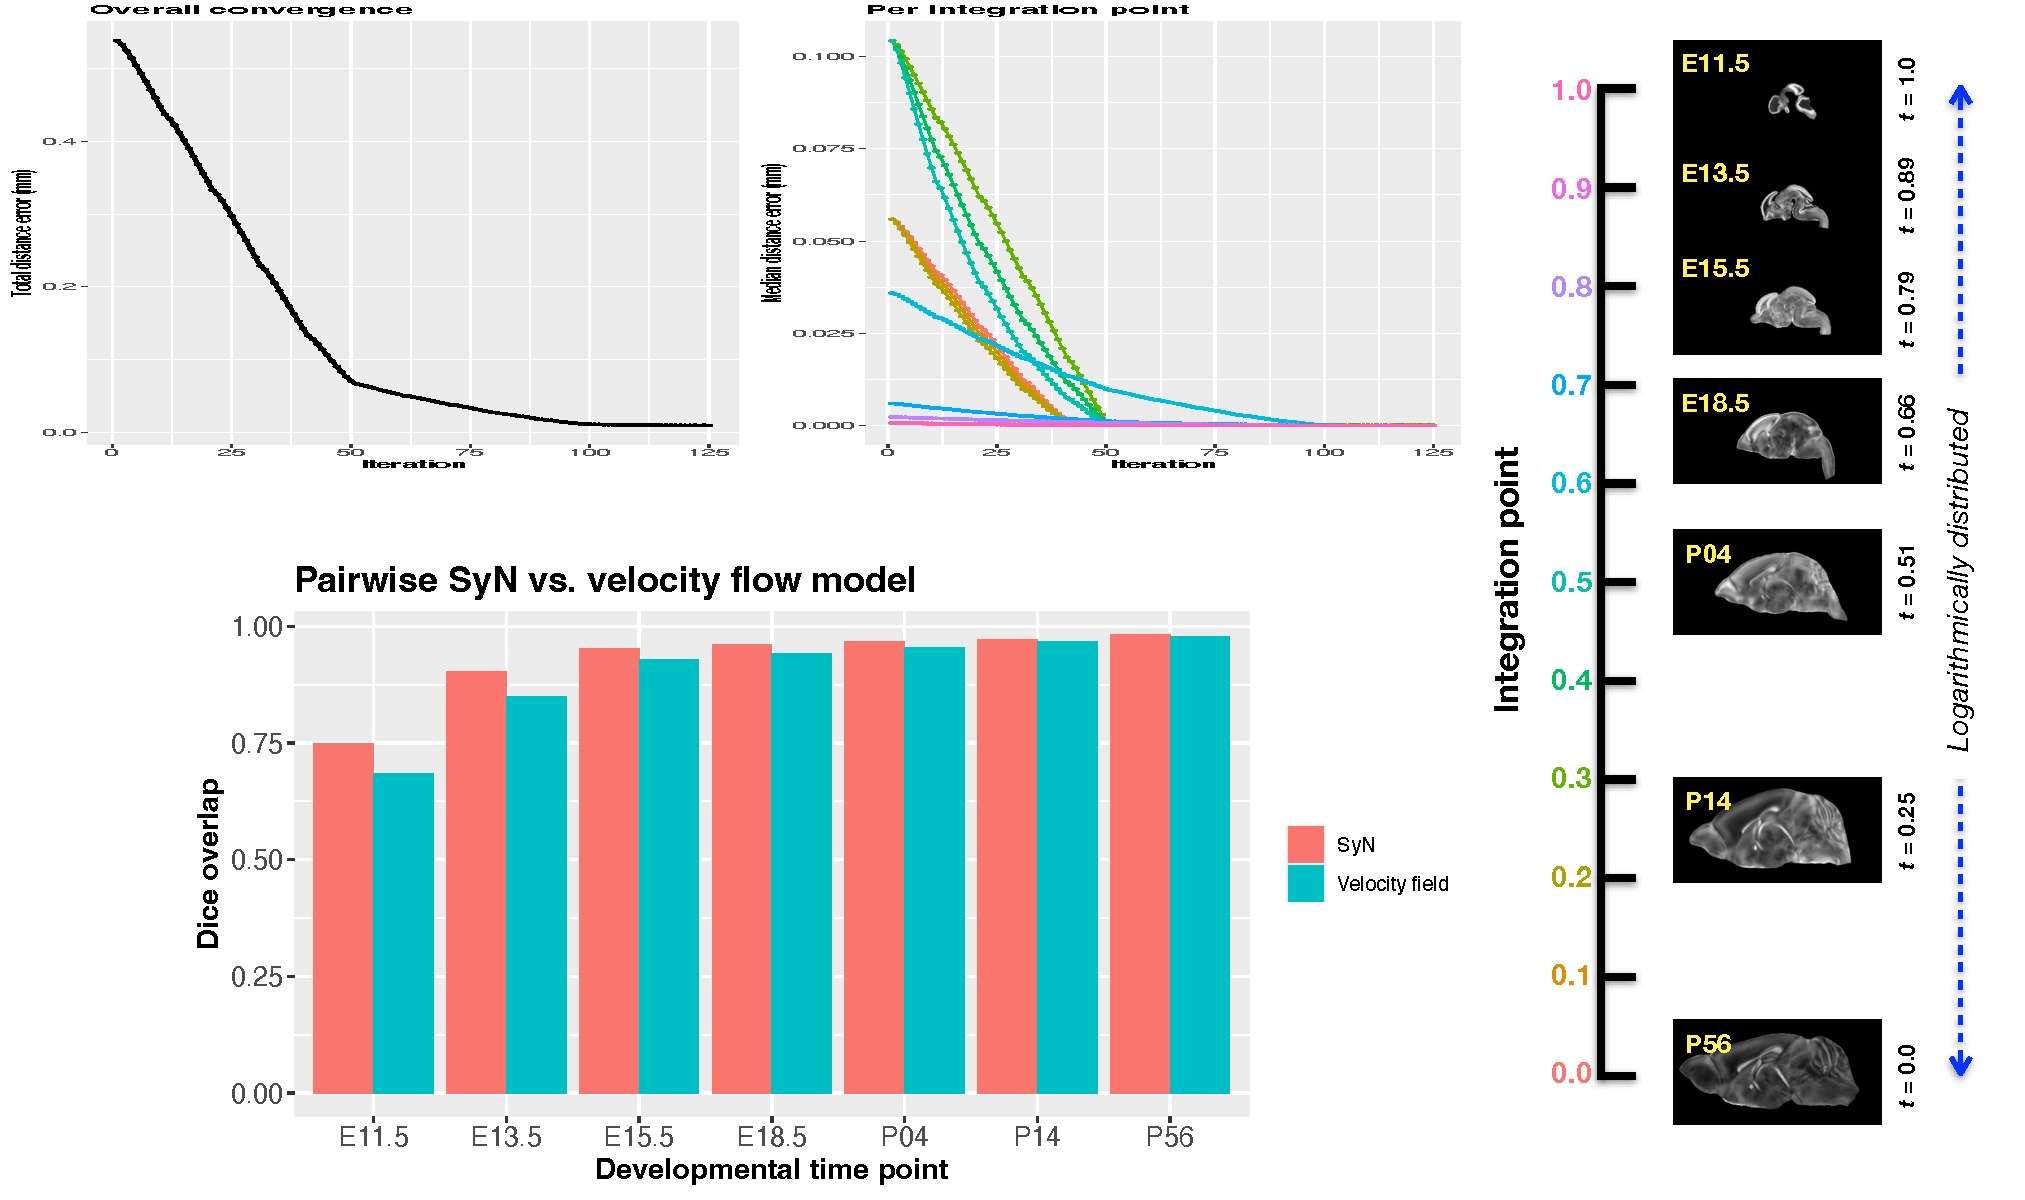
\includegraphics[width=0.99\textwidth]{Figures/convergence.pdf}
\caption{Convergence of the optimization of the velocity field for describing
the transformation through the developmental stages from E11.5 through P56.
Integration points in diagram on the right are color-coordinated with the center
plot and placed in relation to the logarithmically situated temporal placement
of the individual DevCCF atlases.}
\label{fig:convergence}
\end{figure}

The velocity field was optimized using the input composed of the seven
corresponding point sets and their associated weight values, the
selected number of integration points for the velocity field (\(N=11\)),
and the parameters defining the geometry of the spatial dimensions of
the velocity field. Thus, the optimized velocity field described here is
of size \([256, 182, 360]\) (\(50
\mu\)m isotropic) \(\times 11\) integration points for a total
compressed size of a little over 2 GB. This choice represented weighing
the trade-off between tractability, portability, and accuracy. However,
all data and code to reproduce the results described are available in
the dedicated GitHub repository.

The normalized time point scalar value for each atlas/point-set in the
temporal domains \([0, 1]\) was also defined. Given the increasingly
larger gaps in the postnatal time point sampling, we made two
adjustments. Based on known mouse brain development, we used 28 days for
the P56 data. We then computed the log transform of the adjusted set of
time points prior to normalization between 0 and 1 (see the right side
of Figure \ref{fig:convergence}). This log transform, as part of the
temporal normalization, significantly improves the temporal spacing of
data.

The maximum number of iterations was set to 200 with each iteration
taking approximately six minutes on a 2020 iMac (processor, 3.6 GHz
10-Core Intel Core i9; memory, 64 GB 2667 MHz DDR4) At each iteration we
looped over the 11 integration points. At each integration point, the
velocity field estimate was updated by warping the two immediately
adjacent point sets to the integration time point and determining the
regularized displacement field between the two warped point sets. As
with any gradient-based descent algorithm, this field was multiplied by
a small step size (\(\delta = 0.2\)) before adding to the current
velocity field. Convergence is determined by the average displacement
error over each of the integration points. As can be seen in the left
panel of Figure \ref{fig:convergence}, convergence occurred around 125
iterations when the average displacement error over all integration
points is minimized. The median displacement error at each of the
integration points also trends towards zero but at different rates.

\subsubsection{The velocity flow transformation
model}\label{the-velocity-flow-transformation-model}

\begin{figure}[!htb]
\centering
\includegraphics[width=0.8\textwidth]{Figures/CrossWarp.pdf}
\caption{Mid-sagittal visualization of the effects of the transformation model in
warping every developmental stage to the time point of every other developmental
stage.  The original images are located along the diagonal.  Columns correspond
to the warped original image whereas the rows represent the reference space to which
each image is warped.}
\label{fig:crosswarp}
\end{figure}

\begin{figure}[!htb]
\centering
\includegraphics[width=0.8\textwidth]{Figures/pseudo_template.pdf}
\caption{Illustration of the use of the velocity flow model for creating virtual templates
at continuous time points not represented in one of the existing DevCCF time points.
For example, FA templates at time point P10.3 and P20 can be generated by warping the 
existing temporally adjacent developmental templates to the target time point and using 
those images in the ANTsX template building process.}
\label{fig:virtual}
\end{figure}

Once optimized, the resulting velocity field can be used to generate the
deformable transform between any two continuous points within the time
interval bounded by E11.5 and P56. As a demonstration, in Figure
\ref{fig:crosswarp}, we transform each atlas to the space of every other
atlas using the DevCCF transform model. Additionally, one can use this
transformation model to construct virtual templates in the temporal gaps
of the DevCCF. Given an arbitrarily chosen time point within the
normalized time point interval, the existing adjacent DevCCF atlases on
either chronological side can be warped to the desired time point. A
subsequent call to one of the ANTsX template building functions then
permits the construction of the template at that time point. In Figure
\ref{fig:virtual}, we illustrate the use of the DevCCF velocity flow
model for generating two such virtual templates for two arbitrary time
points. Note that both of these usage examples can be found in the
GitHub repository previously given.

\subsection{Automated structural parcellations of the mouse
brain}\label{automated-structural-parcellations-of-the-mouse-brain-1}

\begin{figure}
\centering
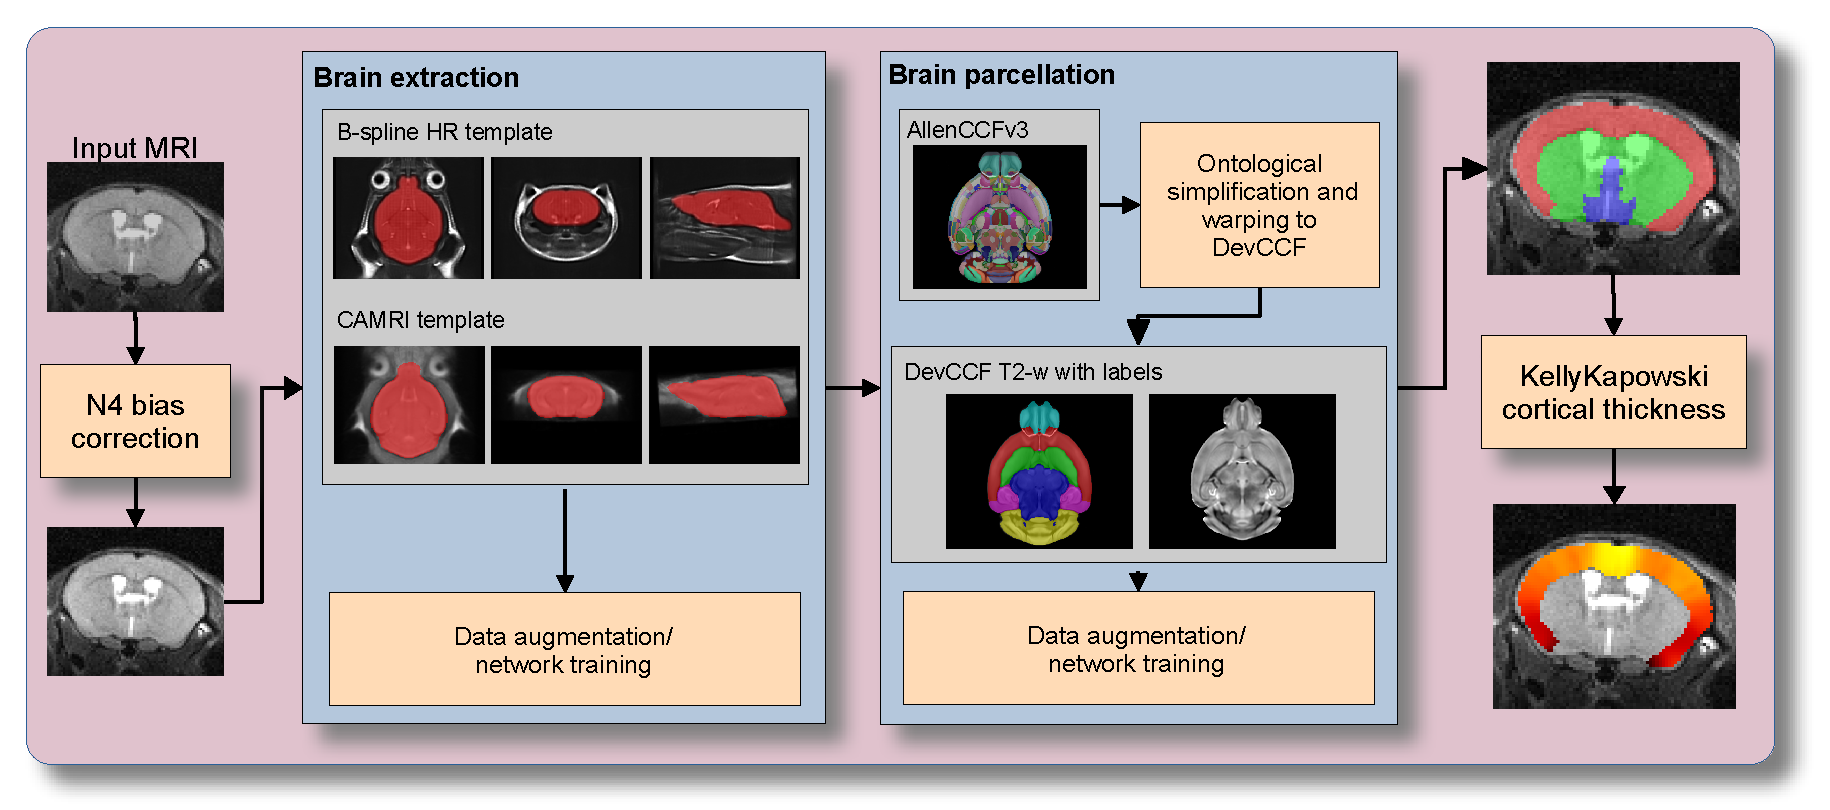
\includegraphics[width=0.95\textwidth]{Figures/mousePipeline.pdf}
\caption{The mouse brain cortical parcellation pipeline integrating two deep
learning components for brain extraction and brain parcellation prior to
estimating cortical labels. Both deep learning networks rely heavily on
aggressive data augmentation on templates built from open data and provide an
outline for further refinement and creating alternative parcellations for
tailored research objectives.  Possible applications include
voxelwise cortical thickness measurements.}
\label{fig:mouseKK}
\end{figure}

Brain parcellation strategies for the mouse brain are pivotal for
understanding the complex organization and function of murine nervous
system\textsuperscript{82}. By dividing the brain into distinct regions
based on anatomical, physiological, or functional characteristics,
researchers can investigate specific areas in isolation and identify
their roles in various behaviors and processes. For example, such
parcellation schemes can help elucidate the spatial distribution of gene
expression patterns\textsuperscript{83} as well as identify functional
regions involved in specific cognitive tasks\textsuperscript{84}.

Although deep learning techniques have been used to develop useful
parcellation tools for human brain research (e.g.,
SynthSeg\textsuperscript{85}, ANTsXNet\textsuperscript{46}), analogous
development for the mouse brain is limited. In addition, mouse data is
often characterized by unique imaging issues such as extreme anisotropic
sampling which are often in sharp contrast to the high resolution
template-based resources available within the community, e.g.,
AllenCCFv3 and DevCCF. We demonstrate how one can use the ANTsX tools to
develop a complete mouse brain structural morphology pipeline as
illustrated in Figure \ref{fig:mouseKK} and detailed below.

\subsubsection{Few-shot mouse brain extraction
network}\label{few-shot-mouse-brain-extraction-network}

In order to create a generalized mouse brain extraction network, we
built whole-head templates from two publicly available datasets. The
Center for Animal MRI (CAMRI) dataset\textsuperscript{69} from the
University of North Carolina at Chapel Hill consists of 16 T2-w MRI
volumes of voxel resolution \(0.16
\times 0.16 \times 0.16 mm^3\). The second high-resolution
dataset\textsuperscript{70} comprises 88 specimens each with three
spatially aligned canonical views with in-plane resolution of
\(0.08 \times 0.08 mm^2\) with a slice thickness of \(0.5 mm\). These
three orthogonal views were used to reconstruct a single high-resolution
volume per subject using a B-spline fitting algorithm available in
ANTsX\textsuperscript{86}.

From these two datasets, two ANTsX templates\textsuperscript{60} were
generated. Bias field simulation, intensity histogram warping, noise
simulation, random translation and warping, and random anisotropic
resampling in the three canonical directions were used for data
augmentation in training an initial T2-w brain extraction network. This
network was posted and the corresponding functionality was immediately
made available within ANTsXNet, similar to our previous contributions to
the community.

User interest led to a GitHub inquiry regarding possible study-specific
improvements (\url{https://github.com/ANTsX/ANTsPyNet/issues/133}). This
interaction led to the offering of a user-made third template and
extracted brian mask generated from T2-w ex-vivo data with isotropic
spacing of 0.08 mm in each voxel dimension. This third template, in
conjunction with the other two, were used with the same aggressive data
augmentation to refine the network weights which were subsequently
posted and made available through ANTsPyNet using the function
\texttt{antspynet.mouse\_brain\_extraction(...)}.

\subsubsection{Single-shot mouse brain parcellation
network}\label{single-shot-mouse-brain-parcellation-network}

AllenCCFv3 and its hierarchical ontological labeling, along with the
DevCCF, provides the necessary data for developing a tailored structural
parcellation network for multi-modal imaging. The \texttt{allensdk}
Python library permits the creation of any gross parcellation based on
the AllenCCFv3 ontology. Specifically, using \texttt{allensdk} we
coalesced the labels to the following six major structures: cerebral
cortex, cerebral nuclei, brain stem, cerebellum, main olfactory bulb,
and hippocampal formation. This labeling was mapped to the P56 component
of the DevCCF for use with the T2-w template component.

The T2-w P56 DevCCF and labelings, in conjunction with the data
augmentation described previously for brain extraction, were used to
train the proposed brain parcellation network. This is available in
ANTsXNet (e.g.~in ANTsPyNet using
\texttt{antspynet.mouse\_brain\_parcellation(...)}). Note that other
brain parcellation networks have also been trained using alternative
regions and parcellation schemes and are available in the same ANTsXNet
functionality. One usage note is that the data augmentation used to
train the network permits a learned interpolation in 0.08 mm isotropic
space. Since the training data is isotropic and data augmentation
includes downsampling in the canonical directions, each of the two
networks learns mouse brain-specific interpolation such that one can
perform prediction on thick-sliced images, as, for example, in these
evaluation data, and return isotropic probability and thickness maps (a
choice available to the user). This permits robust cortical thickness
estimation even in the case of anisotropic data (see
\texttt{antspynet.mouse\_cortical\_thickness(...)}).

\subsubsection{Evaluation}\label{evaluation}

\begin{figure}
\centering
  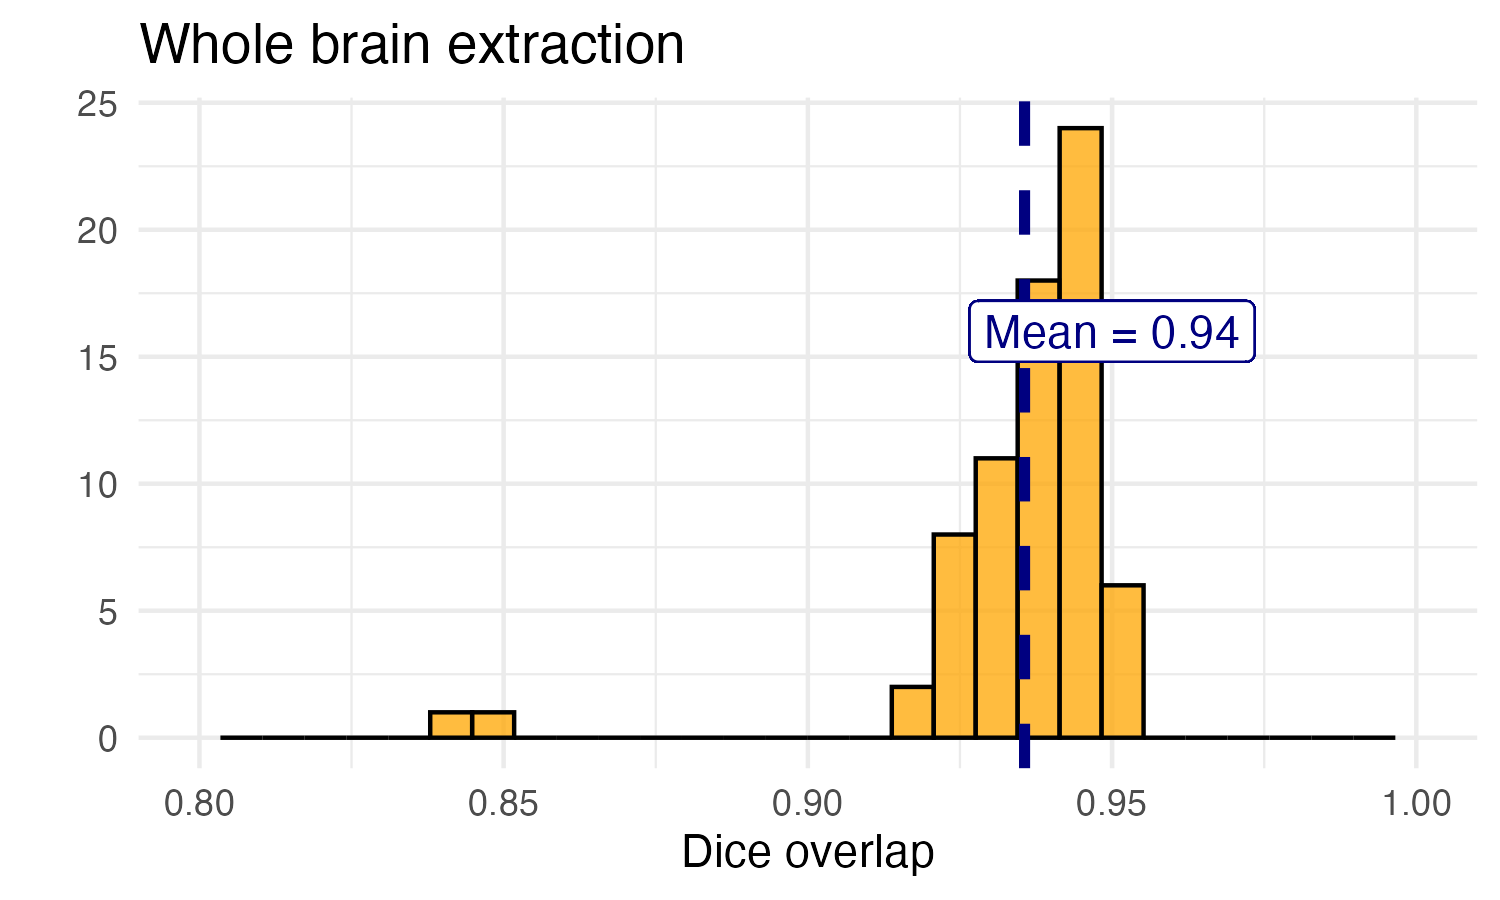
\includegraphics[width=0.75\textwidth]{Figures/diceWholeBrain.png}
\caption{Evaluation of the ANTsX mouse brain extraction on an
independent, publicly available dataset consisting of 12 specimens $\times$ 7
time points = 84 total images.  Dice overlap comparisons with the
user-generated brain masks provide good agreement with the automated results
from the brain extraction network.}
\label{fig:evaluation}
\end{figure}

\begin{figure}
\centering
\begin{subfigure}{0.25\textwidth}
  \centering
  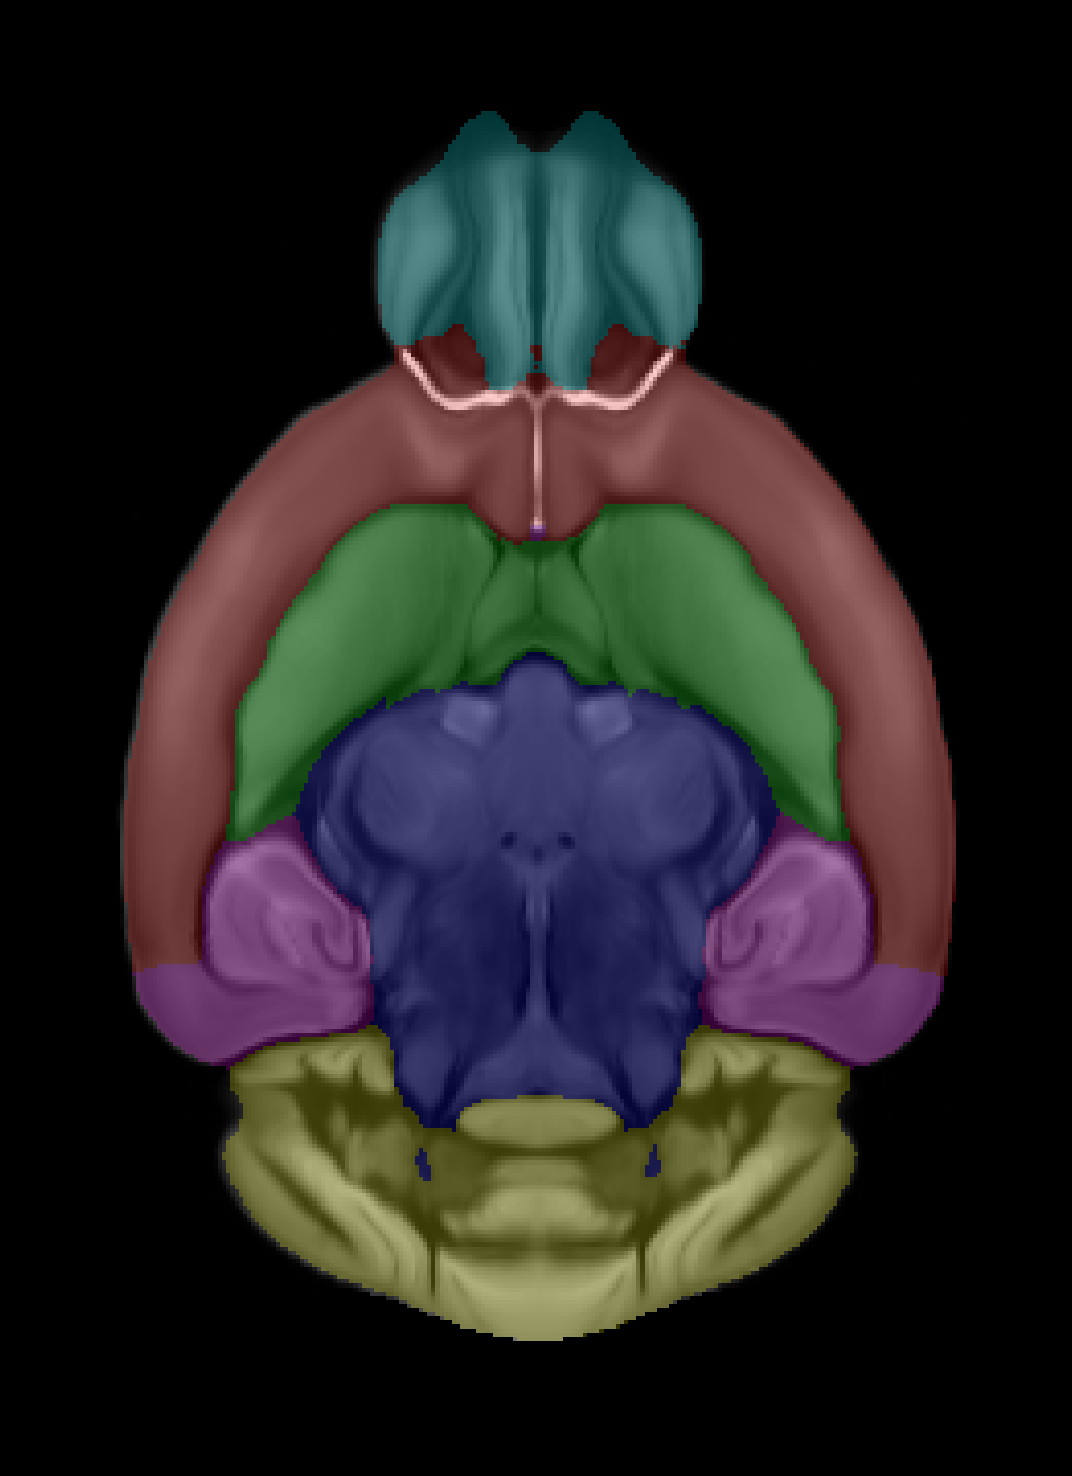
\includegraphics[width=\linewidth]{Figures/AllenCCFv3_parcellation_slice91.png}
  \caption{}
  \label{fig:subp_a}
\end{subfigure}
\begin{subfigure}{0.25\textwidth}
  \centering
  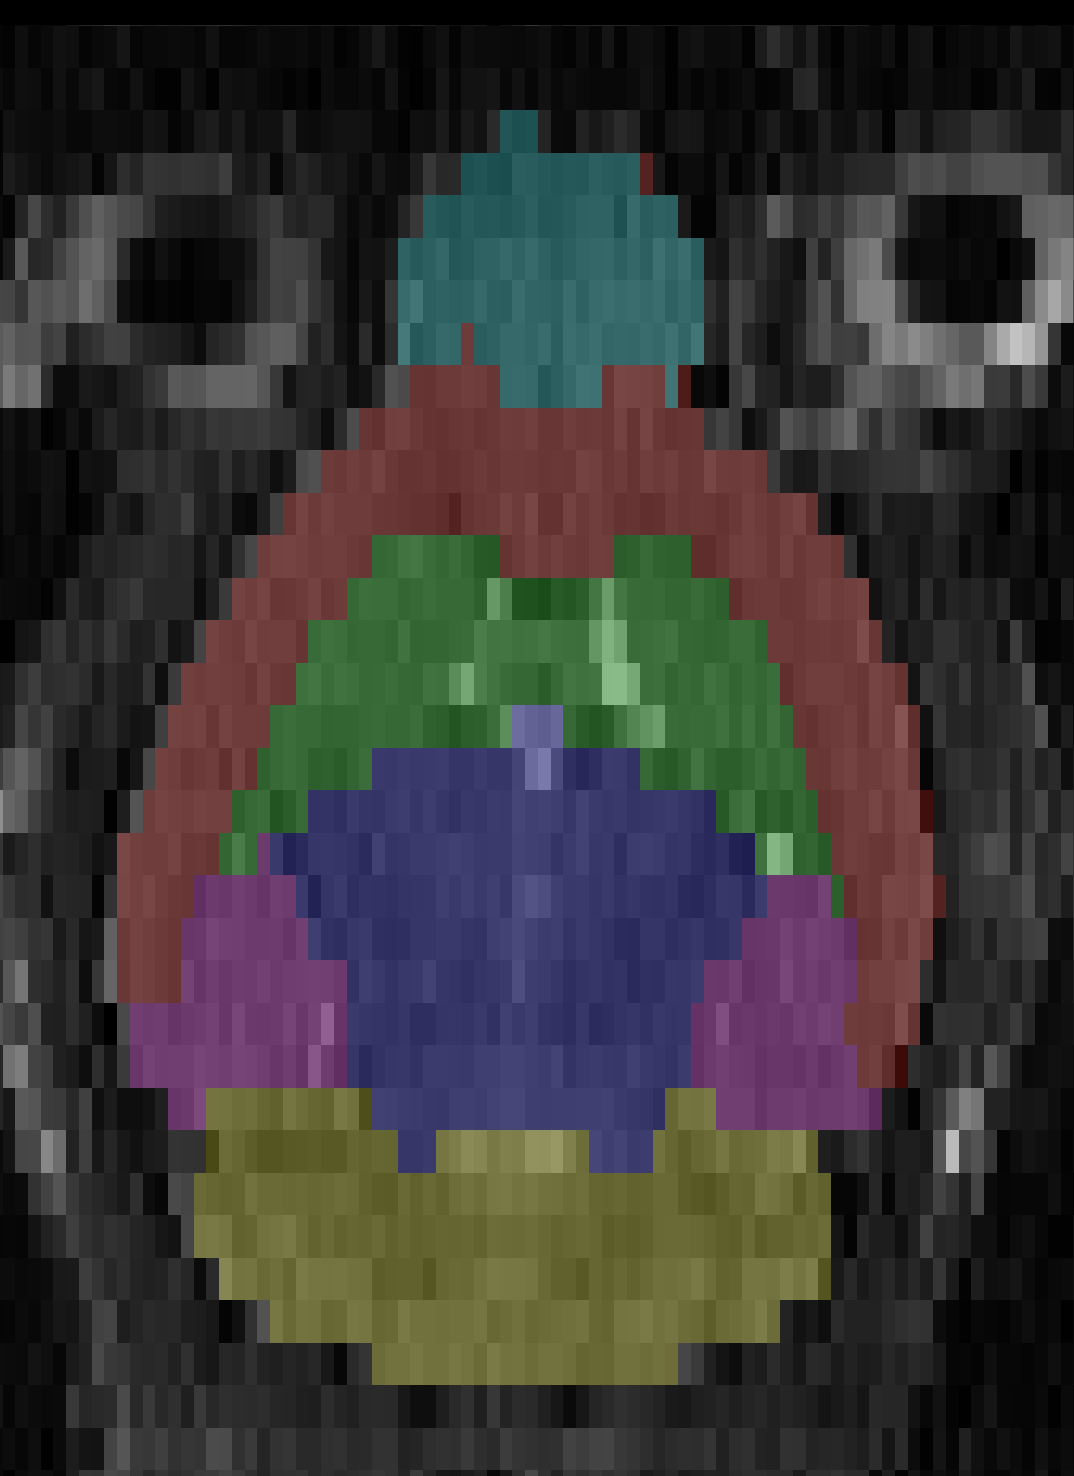
\includegraphics[width=\linewidth]{Figures/NR5_M_Day0_slice53.png}
  \caption{}
  \label{fig:subp_b}
\end{subfigure} \\
\begin{subfigure}{.75\textwidth}
  \centering
  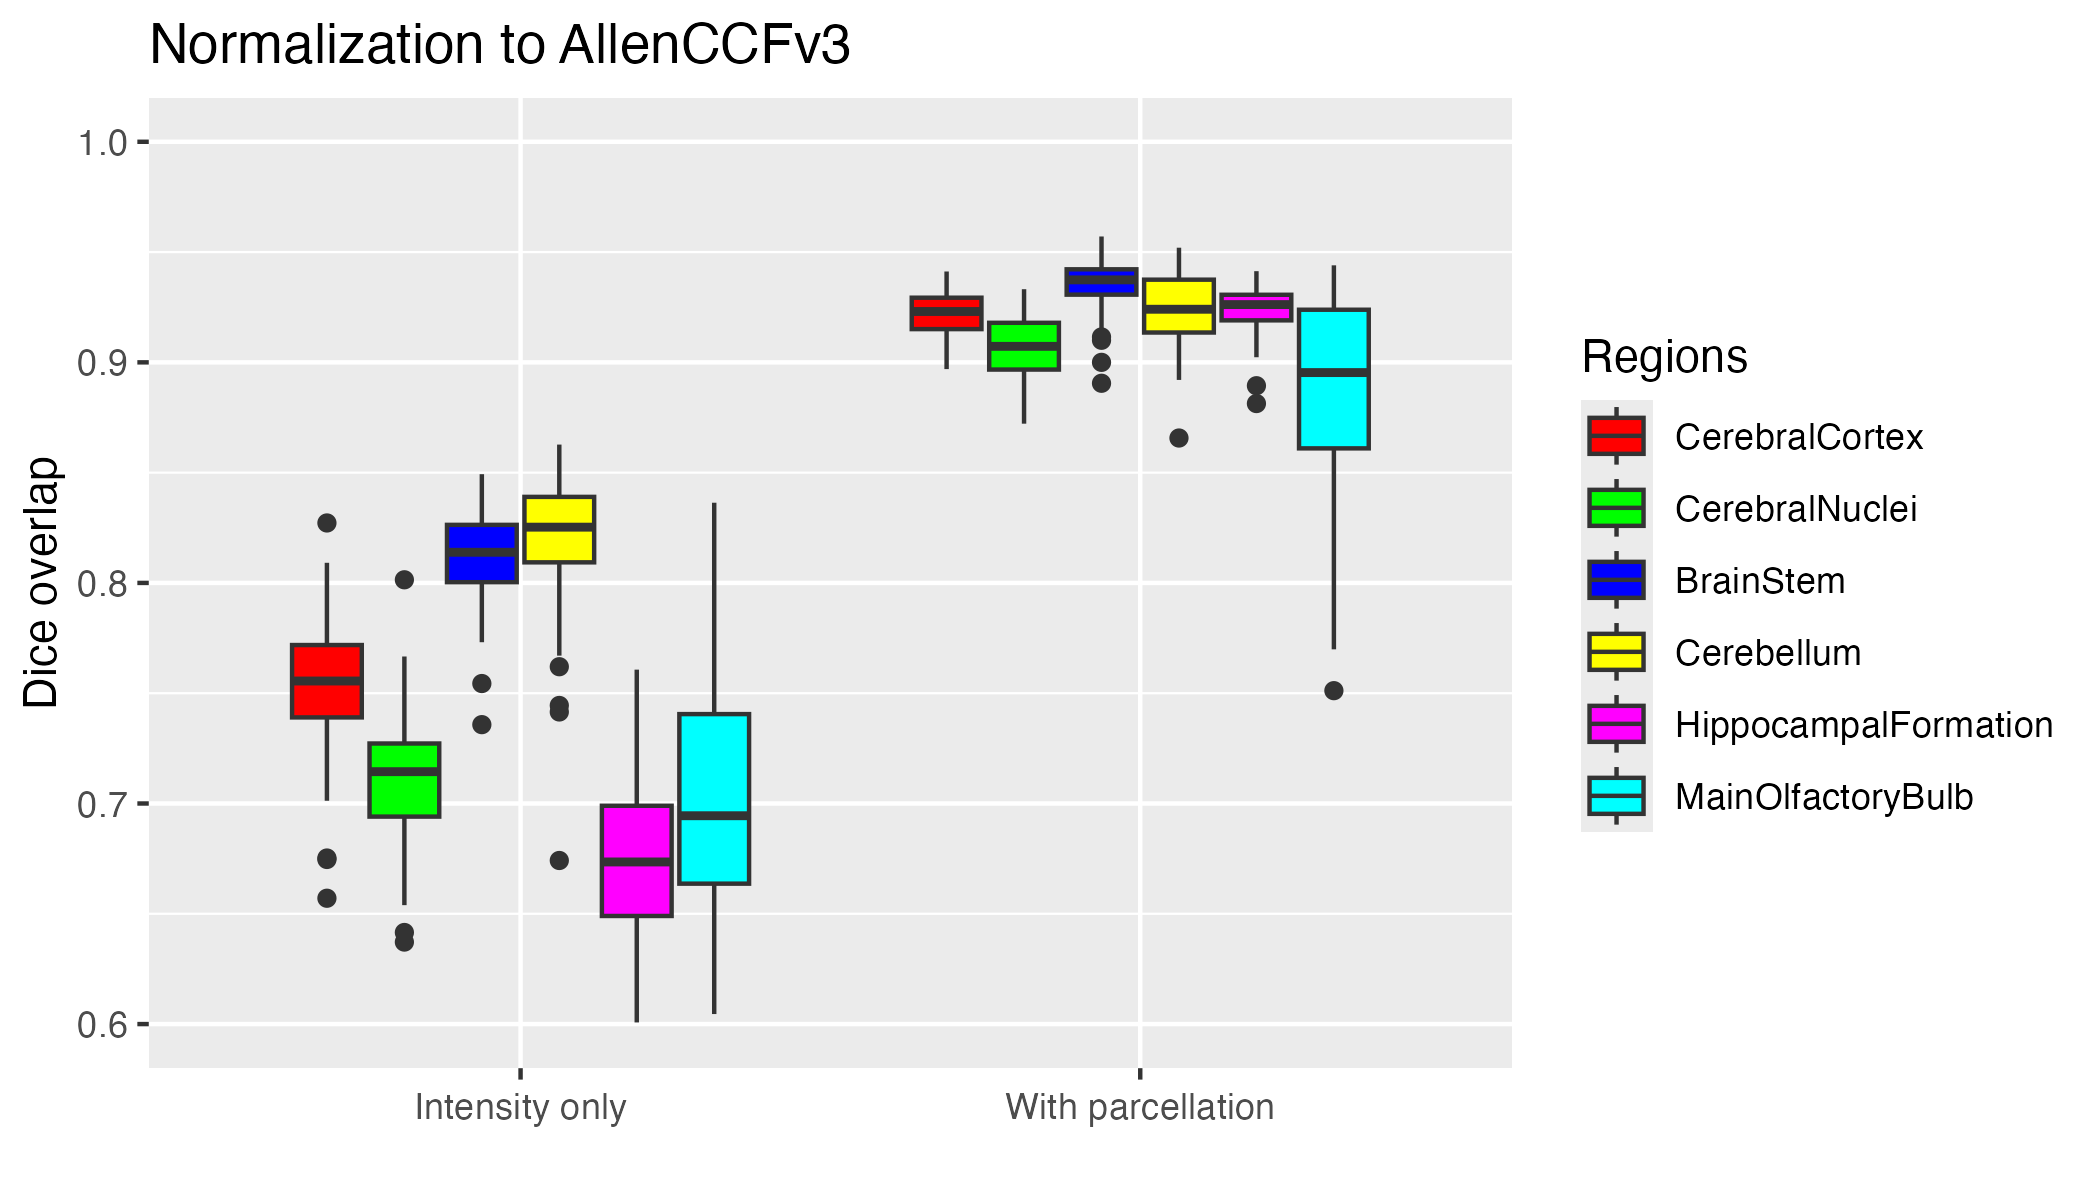
\includegraphics[width=\linewidth]{Figures/diceAllenCCFv3.png}
  \caption{}
  \label{fig:subc}
\end{subfigure}
\caption{Evaluation of the ANTsX mouse brain parcellation on the same dataset.
(a) T2-w DevCCF P56 with the described parcellation consisting of the cerebral
cortex, nuclei, brain stem, cerebellum, main olfactory bulb, and hippocampal
formation. (b) Sample subject (NR5 Day 0) with the proposed deep learning-based
segmentation. (c) Dice overlap for comparing the regional alignments between
registration using intensity information only and using intensity with the given
parcellation scheme.}
\label{fig:evaluationParcellation}
\end{figure}

For evaluation, we used an additional publicly available
dataset\textsuperscript{71} that is completely independent from the data
used in training the brain extraction and parcellation networks. Data
includes 12 specimens each imaged at seven time points (Day 0, Day 3,
Week 1, Week 4, Week 8, Week 20) with in-house-generated brain masks for
a total of 84 images. Spacing is anistropic with an in-plane resolution
of \(0.1 \times 0.1 mm^2\) and a slice thickness of \(0.5 mm\).

Figure \ref{fig:evaluation} summarizes the whole brain overlap between
the provided segmentations for all 84 images and the results of applying
the proposed network. Also, since mapping to the AllenCCFv3 atlas is
crucial for many mouse studies, we demonstrate the utility of the second
network by leveraging the labeled regions to perform
anatomically-explicit alignment using ANTsX multi-component registration
instead of intensity-only registration. For these data, the whole brain
extraction demonstrates excellent performance across the large age
range. And although the intensity-only image registration provides
adequate alignment, intensity with the regional parcellations
significantly improves those measures.

\clearpage
\newpage

\section{Discussion}\label{discussion}

The diverse mouse brain cell type profiles gathered through BICCN and
associated efforts provides a rich multi-modal resource to the research
community. However, despite significant progress, optimized leveraging
of these valuable resources is ongoing. A central component to data
integration is accurately mapping novel cell type data into CCFs for
subsequent processing and analysis. To meet these needs, tools for
mapping mouse cell type data must be both generally accessible to a wide
audience of investigators, and capable of handling distinct challenges
unique to each data type. In this work, we described modular ANTsX-based
pipelines developed to address the needs of three BICCN projects that
cover distinct cell type data, including spatial transcriptomic,
morphological, and developmental data. We highlighted how a modular
toolbox like ANTsX can be tailored to address problems unique to each
modality through leveraging a variety of ready-to-use powerful tools
that have been previously validated in multiple application scenarios.

Our MERFISH pipeline provides an example of how to map high-resolution
spatial transcriptomic data into the AllenCCFv3. While the techniques
employed for mapping the sectioned data can be generally applicable to
spatially transform other serial histology images, much of the pipeline
was designed to specifically address known alignment challenges in the
MERFISH data. Thus pipeline shows how general ANTsX tools can be adapted
to target highly specialized problems in mouse cell type data.

In contrast to the MERFISH pipeline, our fMOST pipeline was designed to
be a more general solution that can be employed in other modalities. The
pipeline primarily uses previously developed ANTsX preprocessing and
atlasing tools to map fMOST data into the AllenCCFv3. The key component
of the pipeline is the use of a fMOST-specific average shape and
intensity atlas to most effectively address image registration in this
context. The mapping between the fMOST atlas is generated once and
reused for each new fMOST image. Lastly, ANTsX provides point set
transformation tools to allow the mappings found through the pipeline to
be directly applied to associated single-cell reconstructions from the
fMOST data to study neuronal morphology.

The pipeline for continuously mapping the DevCCF data is also available
in ANTsX and is generally applicable for spatio-temporal mapping. With
specific application to the DevCCF, despite the significant expansion of
available developmental age templates beyond what existed previously,
there are still temporal gaps in the DevCCF which can be potentially
sampled by future research efforts. However, pioneering work involving
time-varying diffeomorphic transformations allow us to continuously
situate the existing templates within a velocity flow model. This allows
one to determine the diffeomorphic transformation from any one temporal
location to any other temporal location within the time span defined by
the temporal limits of the DevCCF. This functionality is built on
multiple ITK components including the B-spline scattered data
approximation technique for field regularization and velocity field
integration. This velocity field model permits intra-template comparison
and the construction of virtual templates where a template can be
estimated at any continuous time point within the temporal domain. This
novel application can potentially enhance our understanding of
intermediate developmental stages.

We also presented a mouse brain morphological pipeline for brain
extraction and brain parcellation using single-shot and few-shot
learning with aggressive data augmentation. This approach attempts to
circumvent (or at least minimize) the typical requirement of large
training datasets as with the human ANTsX pipeline analog. However, even
given our initial success on independent data, we anticipate that
refinements will be necessary. Given that the ANTsX toolkit is a dynamic
effort undergoing continual improvement, we manually correct cases that
fail and use them for future training and refinement of network weights
as we have done for our human-based networks. And, as demonstrated, we
welcome contributions from the community for improving these approaches
which, generally, provide a way to bootstrap training data for manual
refinement and future generation of more accurate deep learning networks
in the absence of other applicable tools.

The ANTsX ecosystem is a powerful framework that has demonstrated
applicability to diverse cell type data in the mouse brain. This is
further evidenced by the many software packages that use various ANTsX
components in their own mouse-specific workflows. The extensive
functionality of ANTsX makes it possible to create complete processing
pipelines without requiring the integration of multiple packages or
lengthy software development. These open-source components not only
perform well but are available across multiple platforms which
facilitates the construction of tailored pipelines for individual study
solutions. These components are also supported by years of development
not only by the ANTsX development team but by the larger ITK community.
Finally, as an extension to the BICCN program, ANTsX will be a powerful
tool for the efforts of the BRAIN Initiative Cell Atlas Network (BICAN)
to extend these efforts to the human brain.

\clearpage
\newpage

\section{Methods}\label{methods}

The following methods are all available as part of the ANTsX ecosystem
with analogous elements existing in both ANTsR (ANTs in R) and ANTsPy
(ANTs in Python) with an ANTs/ITK C++ core. However, most of the
development for the work described below was performed using ANTsPy. For
equivalent calls in ANTsR, please see the ANTsX tutorial at
\url{https://tinyurl.com/antsxtutorial}.

\subsection{General ANTsX utilities}\label{general-antsx-utilities}

Although they focus on distinct data types, the three pipelines
presented share common components that are generally applicable when
mapping mouse cell type data. These include, addressing intensity biases
and noise in the data, image registration to solve the mapping, creating
custom templates and atlases from the data, and visualization of the
results. Table \ref{table:methods} provides a brief summary of key
general functionalities in ANTsX for addressing these challenges.


\begin{table}
  \small
   \centering
   \vspace{-0.25cm}
   \caption{Sampling of ANTsX functionality} 
   \begin{tabular*}{0.95\textwidth}{l @{\extracolsep{\fill}} p{.575\textwidth}}
    \toprule
    \multicolumn{2}{c}{\cellcolor{gray!25} \em ANTsPy: Preprocessing} \\
    \cmidrule[1pt](lr){1-2}
    bias field correction & \texttt{n4\_bias\_field\_correction(...)} \\
    image denoising  & \texttt{denoise\_image(...)} \\
    \cmidrule[1pt](lr){1-2}
    \multicolumn{2}{c}{\cellcolor{gray!25} \em ANTsPy: Registration} \\
    \cmidrule[1pt](lr){1-2}
    image registration & \texttt{registration(...)} \\
    image transformation & \texttt{apply\_transforms(...)} \\
    template generation  & \texttt{build\_template(...)} \\
    landmark registration & \texttt{fit\_transform\_to\_paired\_points(...)} \\
    time-varying landmark reg. & \texttt{fit\_time\_varying\_transform\_to\_point\_sets(...)} \\
    integrate velocity field & \texttt{integrate\_velocity\_field(...)} \\
    invert displacement field & \texttt{invert\_displacement\_field(...)} \\
    \cmidrule[1pt](lr){1-2}
    \multicolumn{2}{c}{\cellcolor{gray!25} \em ANTsPy: Segmentation} \\
    \cmidrule[1pt](lr){1-2}
    MRF-based segmentation & \texttt{atropos(...)} \\
    Joint label fusion & \texttt{joint\_label\_fusion(...)} \\
    diffeormorphic thickness   & \texttt{kelly\_kapowski(...)} \\
    \cmidrule[1pt](lr){1-2}
    \multicolumn{2}{c}{\cellcolor{gray!25} \em ANTsPy: Miscellaneous} \\
    \cmidrule[1pt](lr){1-2}
    Regional intensity statistics & \texttt{label\_stats(...)} \\
    Regional shape measures & \texttt{label\_geometry\_measures(...)} \\
    B-spline approximation & \texttt{fit\_bspline\_object\_to\_scattered\_data(...)} \\
    Visualize images and overlays\,\,\,\,\,\,\,\,\,\,\,\, & \texttt{plot(...)} \\
    \cmidrule[1pt](lr){1-2}
    \multicolumn{2}{c}{\cellcolor{gray!25} \em ANTsPyNet: Mouse-specific} \\
    \cmidrule[1pt](lr){1-2}
    brain extraction & \texttt{mouse\_brain\_extraction(...modality="t2"...)} \\
    brain parcellation & \texttt{mouse\_brain\_parcellation(...)}  \\
    cortical thickness & \texttt{mouse\_cortical\_thickness(...)}  \\
    % foreground extraction & \texttt{mouse\_histology\_brain\_mask(...)} \\
    % midline segmentation & \texttt{mouse\_histology\_hemispherical\_coronal\_mask(...)} \\
    % cerebellum segmentation & \texttt{mouse\_histology\_cerebellum\_mask(...)} \\
    super resolution & \texttt{mouse\_histology\_super\_resolution(...)} \\
    \bottomrule
    \multicolumn{2}{l}{\makecell[l]{
     \vspace{-3pt}
     \scriptsize ANTsX provides state-of-the-art functionality for processing biomedical image data.  Such tools, including deep \\
     \vspace{-3pt}
     \scriptsize learning networks, support a variety of mapping-related tasks.  A more comprehensive listing of ANTsX tools with \\
     \vspace{-3pt}
     \scriptsize self-contained R and Python examples is provided as a gist page on GitHub (\url{https://tinyurl.com/antsxtutorial}). }
    }
   \end{tabular*}
 \label{table:methods}
\end{table}


\subsubsection{Preprocessing: bias field correction and
denoising}\label{preprocessing-bias-field-correction-and-denoising}

Bias field correction and image denoising are standard preprocessing
steps in improving overall image quality in mouse brain images. The bias
field, a gradual spatial intensity variation in images, can arise from
various sources such as magnetic field inhomogeneity or acquisition
artifacts, leading to distortions that can compromise the quality of
brain images. Correcting for bias fields ensures a more uniform and
consistent representation of brain structures, enabling more accurate
quantitative analysis. Additionally, brain images are often susceptible
to various forms of noise, which can obscure subtle features and affect
the precision of measurements. Denoising techniques help mitigate the
impact of noise, enhancing the signal-to-noise ratio and improving the
overall image quality. The well-known N4 bias field correction
algorithm\textsuperscript{53} has its origins in the ANTs toolkit which
was implemented and introduced into the ITK toolkit,
i.e.~\texttt{ants.n4\_bias\_field\_correction(...)}. Similarly, ANTsX
contains an implementation of a well-performing patch-based denoising
technique\textsuperscript{62} and is also available as an image filter
to the ITK community, \texttt{ants.denoise\_image(...)}.

\subsubsection{Image registration}\label{image-registration}

The ANTs registration toolkit is a complex framework permitting highly
tailored solutions to pairwise image registration
scenarios\textsuperscript{87}. It includes innovative transformation
models for biological modeling\textsuperscript{52,68} and has proven
capable of excellent performance\textsuperscript{57,88}. Various
parameter sets targeting specific applications have been packaged with
the different ANTsX packages, specifically ANTs, ANTsPy, and
ANTsR\textsuperscript{46}. In ANTsPy, the function
\texttt{ants.registration(...)} is used to register a pair of images or
a pair of image sets where \texttt{type\_of\_transform} is a
user-specified option that invokes a specific parameter set. For example
\texttt{type\_of\_transform=\textquotesingle{}antsRegistrationSyNQuick{[}s{]}\textquotesingle{}}
encapsulates an oft-used parameter set for quick registration whereas
\texttt{type\_of\_transform=\textquotesingle{}antsRegistrationSyN{[}s{]}\textquotesingle{}}
is a more aggressive alternative. Transforming images using the derived
transforms is performed via the \texttt{ants.apply\_transforms(...)}
function.

Initially, linear optimization is initialized with center of (intensity)
mass alignment typically followed by optimization of both rigid and
affine transforms using the mutual information similarity metric. This
is followed by diffeomorphic deformable alignment using symmetric
normalization (SyN) with Gaussian\textsuperscript{52} or B-spline
regularization\textsuperscript{68} where the forward transform is
invertible and differentiable. The similarity metric employed at this
latter stage is typically either neighborhood cross-correlation or
mutual information. Note that these parameter sets are robust to input
image type (e.g., light sheet fluorescence microscopy, Nissl staining,
and the various MRI modalities) and are adaptable to mouse image
geometry and scaling. Further details can be found in the various
documentation sources for these ANTsX packages.

\subsubsection{Template generation}\label{template-generation}

ANTsX provides functionality for constructing templates from a set (or
multi-modal sets) of input images as originally
described\textsuperscript{60} and recently used to create the DevCCF
templates\textsuperscript{16}. An initial template estimate is
constructed from an existing subject image or a voxelwise average
derived from a rigid pre-alignment of the image population. Pairwise
registration between each subject and the current template estimate is
performed using the Symmetric Normalization (SyN)
algorithm\textsuperscript{52}. The template estimate is updated by
warping all subjects to the space of the template, performing a
voxelwise average, and then performing a ``shape update'' of this latter
image by warping it by the average inverse deformation, thus yielding a
mean image of the population in terms of both intensity and shape. The
corresponding ANTsPy function is \texttt{ants.build\_template(...)}.

\subsubsection{Visualization}\label{visualization}

To complement the well-known visualization capabilities of R and Python,
e.g., ggplot2 and matplotlib, respectively, image-specific visualization
capabilities are available in the \texttt{ants.plot(...)} function
(Python). These are capable of illustrating multiple slices in different
orientations with other image overlays and label images.

\subsection{Mapping fMOST data to
AllenCCFv3}\label{mapping-fmost-data-to-allenccfv3}

\subsubsection{Preprocessing}\label{preprocessing}

\begin{itemize}
\item
  \emph{Downsampling}. The first challenge when mapping fMOST images
  into the AllenCCFv3 is addressing the resolution scale of the data.
  Native fMOST data from an individual specimen can range in the order
  of terabytes, which leads to two main problems. First, volumetric
  registration methods (particularly those estimating local deformation)
  have high computational complexity and typically cannot operate on
  such high-resolution data under reasonable memory and runtime
  constraints. Second, the resolution of the AllenCCFv3 atlas is much
  lower than the fMOST data, thus the mapping process will cause much of
  the high-resolution information in the fMOST images to be lost
  regardless. Thus, we perform a cubic B-spline downsampling of the
  fMOST data to reduce the resolution of each image to match the
  isotropic 25 \(\mu m\) voxel resolution of the AllenCCFv3 intensity
  atlas using \texttt{ants.resample\_image(...)}. An important detail to
  note is that while the fMOST images and atlas are downsampled, the
  mapping learned during the registration is assumed to be continuous.
  Thus, after establishing the mapping to the AllenCCFv3, we can
  interpolate the learned mapping and apply it directly to the
  high-resolution native data directly to transform any spatially
  aligned data (such as the single-cell neuron reconstructions) into the
  AllenCCFv3.
\item
  \emph{Stripe artifact removal}. Repetitive pattern artifacts are a
  common challenge in fMOST imaging where inhomogeneity during the
  cutting and imaging of different sections can leave stripes of hyper-
  and hypo-intensity across the image. These stripe artifacts can be
  latched onto by the registration algorithm as unintended features that
  are then misregistered to non-analogous structures in the AllenCCFv3.
  We address these artifacts by fitting a 3-D bandstop (notch) filter to
  target the frequency of the stripe patterns and removing them prior to
  the image registration.
\item
  \emph{Inhomogeneity correction}. Regional intensity inhomogeneity can
  also occur within and between sections in fMOST imaging due to
  staining or lighting irregularity during acquisition. Similar to
  stripe artifacts, intensity gradients due to inhomogeneity can be
  misconstrued as features during the mapping and result in matching of
  non-corresponding structures. Our pipeline addresses these intensity
  inhomogeneities using N4 bias field correction\textsuperscript{53},
  \texttt{ants.n4\_bias\_field\_correction(...)}.
\end{itemize}

\subsubsection{Steps for spatial normalization to
AllenCCFv3}\label{steps-for-spatial-normalization-to-allenccfv3}

\begin{enumerate}
\def\labelenumi{\arabic{enumi}.}
\item
  \emph{Average fMOST atlas as an intermediate target}. Due to the
  preparation of the mouse brain for fMOST imaging, the resulting
  structure in the mouse brain has several large morphological
  deviations from the AllenCCFv3 atlas. Most notable of these is an
  enlargement of the ventricles, and compression of cortical structures.
  In addition, there is poor intensity correspondence for the same
  anatomic features due to intensity dissimilarity between imaging
  modalities. We have found that standard intensity-base registration is
  insufficient to capture the significant deformations required to map
  these structures correctly into the AllenCCFv3. We address this
  challenge in ANTsX by using explicitly corresponding parcellations of
  the brain, ventricles and surrounding structures to directly recover
  these large morphological differences. However, generating these
  parcellations for each individual mouse brain is a labor-intensive
  task. Our solution is to create an average atlas whose mapping to
  AllenCCFv3 encapsulates these large morphological differences to serve
  as an intermediate registration point. This has the advantage of only
  needing to generate one set of corresponding annotations which is used
  to register between the two atlas spaces. New images are first aligned
  to the fMOST average atlas, which shares common intensity and
  morphological features and thus can be achieved through standard
  intensity-based registration.
\item
  \emph{Average fMOST atlas construction}. An intensity and shape-based
  contralaterally symmetric average of the fMOST image data is
  constructed from 30 images and their contralateral flipped versions.
  We ran three iterations of the atlas construction using the default
  settings. Additional iterations (up to six) were evaluated and showed
  minimal changes to the final atlas construction, suggesting a
  convergence of the algorithm.
\item
  \emph{fMOST atlas to AllenCCFv3 alignment}. Alignment between the
  fMOST average atlas and AllenCCFv3 was performed using a one-time
  annotation-driven approach. Label-to-label registration is used to
  align 7 corresponding annotations in both atlases in the following: 1)
  brain mask/ventricles, 2) caudate/putamen, 3) fimbria, 4) posterior
  choroid plexus, 5) optic chiasm, 6) anterior choroid plexus, and 7)
  habenular commissure. The alignments were performed sequentially, with
  the largest, most relevant structures being aligned first using coarse
  registration parameters, followed by other structures using finer
  parameters. This coarse-to-fine approach allows us to address large
  morphological differences (such as brain shape and ventricle
  expansion) at the start of registration and then progressively refine
  the mapping using the smaller structures. The overall ordering of
  these structures was determined manually by an expert anatomist, where
  anatomical misregistration after each step of the registration was
  evaluated and used to determine which structure should be used in the
  subsequent iteration to best improve the alignment. The transformation
  from this one-time expert-guided alignment is preserved and used as
  the canonical fMOST atlas to AllenCCFv3 mapping in the pipeline.
\item
  \emph{Alignment of individual fMOST mouse brains}. The canonical
  transformation between the fMOST atlas and AllenCCFv3 greatly
  simplifies the registration of new individual fMOST mouse brains into
  the AllenCCFv3. Each new image is first registered into the fMOST
  average atlas, which shares intensity, modality, and morphological
  characteristics. This allows us to leverage standard, intensity-based
  registration functionality\textsuperscript{87} available in ANTsX to
  perform this alignment. Transformations are then concatenated to the
  original fMOST image to move it into the AllenCCFv3 space using
  \texttt{ants.apply\_transforms(...)}.
\item
  \emph{Transformation of single cell neurons}. A key feature of fMOST
  imaging is the ability to reconstruct and examine whole-brain single
  neuron projections\textsuperscript{80}. Spatial mapping of these
  neurons from individual brains into the AllenCCFv3 allows
  investigators to study different neuron types within the same space
  and characterize their morphology with respect to their
  transcriptomics. Mappings found between the fMOST image and the
  AllenCCFv3 using our pipeline can be applied in this way to fMOST
  neuron reconstruction point set data using
  \texttt{ants.apply\_transforms\_to\_points(..)}.
\end{enumerate}

\subsection{Mapping MERFISH data to
AllenCCFv3}\label{mapping-merfish-data-to-allenccfv3}

\subsubsection{Preprocessing}\label{preprocessing-1}

\begin{itemize}
\item
  \emph{Initial volume reconstruction}. Alignment of MERFISH data into a
  3-D atlas space requires an estimation of anatomical structure within
  the data. For each section, this anatomic reference image was created
  by aggregating the number of detected genetic markers (across all
  probes) within each pixel of a \(10
  \times 10 \mu m^2\) grid to match the resolution of the \(10 \mu m\)
  AllenCCFv3 atlas. These reference image sections are then coarsely
  reoriented and aligned across sections using manual annotations of the
  most dorsal and ventral points of the midline. The procedure produces
  an anatomic image stack that serves as an initialization for further
  global mappings into the AllenCCFv3.
\item
  \emph{Anatomical correspondence labeling}. Mapping the MERFISH data
  into the AllenCCFv3 requires us to establish correspondence between
  the anatomy depicted in the MERFISH and AllenCCFv3 data.
  Intensity-based features in MERFISH data are not sufficiently apparent
  to establish this correspondence, so we need to generate instead
  corresponding anatomical labelings of both images with which to drive
  registration. These labels are already available as part of the
  AllenCCFv3; thus, the main challenge is deriving analogous labels from
  the spatial transcriptomic maps of the MERFISH data. Toward this end,
  we assigned each cell from the scRNA-seq dataset to one of the
  following major regions: cerebellum, CTXsp, hindbrain, HPF,
  hypothalamus, isocortex, LSX, midbrain, OLF, PAL, sAMY, STRd, STRv,
  thalamus and hindbrain. A label map of each section was generated for
  each region by aggregating the cells assigned to that region within a
  \(10 \times 10 \mu m^2\) grid. The same approach was used to generate
  more fine grained region specific landmarks (i.e., cortical layers,
  habenula, IC). Unlike the broad labels which cover large swaths of the
  section these regions are highly specific to certain parts of the
  section. Once cells in the MERFISH data are labeled, morphological
  dilation is used to provide full regional labels for alignment into
  the AllenCCFv3.
\item
  \emph{Section matching}. Since the MERFISH data is acquired as
  sections, its 3-D orientation may not be fully accounted for during
  the volume reconstruction step, due to the particular cutting angle.
  This can lead to obliqueness artifacts in the section where certain
  structures can appear to be larger or smaller, or missing outright
  from the section. To address this, we first use a global alignment to
  match the orientations of the MERFISH sections to the atlas space. In
  our pipeline, this section matching is performed in the reverse
  direction by performing a global affine transformation of the
  AllenCCFv3 into the MERFISH data space, and then resampling digital
  sections from the AllenCCFv3 to match each MERFISH section. This
  approach limits the overall transformation and thus resampling that is
  applied to the MERFISH data, and, since the AllenCCFv3 is densely
  sampled, it also reduces in-plane artifacts that result from missing
  sections or undefined spacing in the MERFISH data.
\end{itemize}

\subsubsection{2.5D deformable, landmark-driven alignment to
AllenCCFv3}\label{d-deformable-landmark-driven-alignment-to-allenccfv3}

After global alignment of the AllenCCFv3 into the MERFISH dataset, 2D
per-section deformable refinements are used to address local differences
between the MERFISH sections and the resampled AllenCCFv3 sections. Nine
registrations were performed in sequence using a single label at each
iteration in the following order: 1) brain mask, 2) isocortex (layer
2+3), 3) isocortex (layer 5), 4) isocortex (layer 6), 5) striatum, 6)
medial habenula, 7) lateral habenula, 8) thalamus, and 9) hippocampus.
This ordering was determined empirically by an expert anatomist who
prioritized which structure to use in each iteration by evaluating the
anatomical alignment from the previous iteration. Global and local
mappings are then all concatenated (with appropriate inversions) to
create the final mapping between the MERFISH data and AllenCCFv3. This
mapping is then used to provide a point-to-point correspondence between
the original MERFISH coordinate space and the AllenCCFv3 space, thus
allowing mapping of individual genes and cell types located in the
MERFISH data to be directly mapped into the AllenCCFv3.

\subsection{DevCCF velocity flow transformation
model}\label{devccf-velocity-flow-transformation-model}

Given multiple, linearly or non-linearly ordered point sets where
individual points across the sets are in one-to-one correspondence, we
developed an approach for generating a velocity flow transformation
model to describe a time-varying diffeomorphic mapping as a variant of
the landmark matching solution. Integration of the resulting velocity
field can then be used to describe the displacement between any two time
points within this time-parameterized domain. Regularization of the
sparse correspondence between point sets is performed using a
generalized B-spline scattered data approximation
technique\textsuperscript{86}, also created by the ANTsX developers and
contributed to ITK.

\subsubsection{Velocity field
optimization}\label{velocity-field-optimization-1}

To apply this methodology to the developmental
templates\textsuperscript{16}, we coalesced the manual annotations of
the developmental templates into 26 common anatomical regions (see
Figure \ref{fig:simplifiedannotations}). We then used these regions to
generate invertible transformations between successive time points.
Specifically each label was used to create a pair of single region
images resulting in 26 pairs of ``source'' and ``target'' images. The
multiple image pairs were simultaneously used to iteratively estimate a
diffeomorphic pairwise transform. Given the seven atlases E11.5, E13.5,
E15.5, E18.5, P4, P14, and P56, this resulted in 6 sets of transforms
between successive time points. Approximately 10\(^6\) points were
randomly sampled labelwise in the P56 template space and propagated to
each successive atlas providing the point sets for constructing the
velocity flow model. Approximately 125 iterations resulted in a steady
convergence based on the average Euclidean norm between transformed
point sets. Ten integration points were used and point sets were
distributed along the temporal dimension using a log transform for a
more evenly spaced sampling. For additional information a help menu is
available for the ANTsPy function
\texttt{ants.fit\_time\_varying\_transform\_to\_point\_sets(...)}.

\subsection{ANTsXNet mouse brain
applications}\label{antsxnet-mouse-brain-applications}

\subsubsection{General notes regarding deep learning
training}\label{general-notes-regarding-deep-learning-training}

All network-based approaches described below were implemented and
organized in the ANTsXNet libraries comprising Python (ANTsPyNet) and R
(ANTsRNet) analogs using the Keras/Tensorflow libraries available as
open-source in ANTsX GitHub repositories. For the various applications,
both share the identically trained weights for mutual reproducibility.
For all GPU training, we used Python scripts for creating custom batch
generators which we maintain in a separate GitHub repository for public
availability (\url{https://github.com/ntustison/ANTsXNetTraining}).
These scripts provide details such as batch size, choice of loss
function, and network parameters. In terms of GPU hardware, all training
was done on a DGX (GPUs: 4X Tesla V100, system memory: 256 GB LRDIMM
DDR4).

Data augmentation is crucial for generalizability and accuracy of the
trained networks. Intensity-based data augmentation consisted of
randomly added noise (i.e., Gaussian, shot, salt-and-pepper), simulated
bias fields based on N4 bias field modeling, and histogram warping for
mimicking well-known MRI intensity
nonlinearities\textsuperscript{46,89}. These augmentation techniques are
available in ANTsXNet (only ANTsPyNet versions are listed with ANTsRNet
versions available) and include:

\begin{itemize}
\item
  image noise: \texttt{ants.add\_noise\_to\_image(...)},
\item
  simulated bias field: \texttt{antspynet.simulate\_bias\_field(...)},
  and
\item
  nonlinear intensity warping:
  \texttt{antspynet.histogram\_warp\_image\_intensities(...)}.
\end{itemize}

Shape-based data augmentation used both random linear and nonlinear
deformations in addition to anisotropic resampling in the three
canonical orientations to mimic frequently used acquisition protocols
for mice brains:

\begin{itemize}
\item
  random spatial warping:
  \texttt{antspynet.randomly\_transform\_image\_data(...)} and
\item
  anisotropic resampling: \texttt{ants.resample\_image(...)}.
\end{itemize}

\subsubsection{Brain extraction}\label{brain-extraction}

Similar to human neuroimage processing, brain extraction is a crucial
preprocessing step for accurate brain mapping. We developed similar
functionality for T2-weighted mouse brains. This network uses a
conventional U-net architecture\textsuperscript{90} and, in ANTsPyNet,
this functionality is available in the program
\texttt{antspynet.mouse\_brain\_extraction(...)}. For the two-shot
T2-weighted brain extraction network, two brain templates were generated
along with their masks. One of the templates was generated from
orthogonal multi-plane, high resolution data\textsuperscript{70} which
were combined to synthesize isotropic volumetric data using the B-spline
fitting algorithm\textsuperscript{86}. This algorithm is encapsulated in
\texttt{ants.fit\_bspline\_object\_to\_scattered\_data(...)} where the
input is the set of voxel intensity values and each associated physical
location. Since each point can be assigned a confidence weight, we use
the normalized gradient value to more heavily weight edge regions.
Although both template/mask pairs are available in the GitHub repository
associated with this work, the synthesized volumetric B-spline
T2-weighted pair is available within ANTsXNet through the calls:

\begin{itemize}
\item
  template:
  \texttt{antspynet.get\_antsxnet\_data("bsplineT2MouseTemplate")} and
\item
  mask:
  \texttt{antspynet.get\_antsxnet\_data("bsplineT2MouseTemplateBrainMask")}.
\end{itemize}

\subsubsection{Brain parcellation}\label{brain-parcellation}

The T2-weighted brain parcellation network is also based on a 3-D U-net
architecture and the T2-w DevCCF P56 template component with extensive
data augmentation, as described previously. Intensity differences
between the template and any brain extracted input image are minimized
through the use of the rank intensity transform
(\texttt{ants.rank\_intensity(...)}). Shape differences are reduced by
the additional preprocessing step of warping the brain extracted input
image to the template. Additional input channels include the prior
probability images created from the template parcellation. These images
are also available through the ANTsXNet
\texttt{get\_antsxnet\_data(...)} interface.

\clearpage

\section*{Data availability}\label{data-availability}
\addcontentsline{toc}{section}{Data availability}

All data and software used in this work are publicly available. The
DevCCF atlas is available at \url{https://kimlab.io/brain-map/DevCCF/}.
ANTsPy, ANTsR, ANTsPyNet, and ANTsRNet are available through GitHub at
the ANTsX Ecosystem (\url{https://github.com/ANTsX}). Training scripts
for all deep learning functionality in ANTsXNet can also be found on
GitHub (\url{https://github.com/ntustison/ANTsXNetTraining}). A GitHub
repository specifically pertaining to the AllenCCFv3 mapping is
available at \url{https://github.com/dontminchenit/CCFAlignmentToolkit}.
For the other two contributions contained in this work, the longitudinal
DevCCF mapping and mouse cortical thickness pipeline, we refer the
interested reader to
\url{https://github.com/ntustison/ANTsXMouseBrainMapping}.

\clearpage

\section*{Acknowledgments}\label{acknowledgments}
\addcontentsline{toc}{section}{Acknowledgments}

Support for the research reported in this work includes funding from the
National Institute of Biomedical Imaging and Bioengineering
(R01-EB031722) and National Institute of Mental Health (RF1-MH124605 and
U24-MH114827).

We also acknowledge the data contribution of Dr.~Adam Raikes (GitHub
@araikes) of the Center for Innovation in Brain Science at the
University of Arizona for refining the weights of the mouse brain
extraction network.

\clearpage

\section*{Author contributions}\label{author-contributions}
\addcontentsline{toc}{section}{Author contributions}

N.T., M.C., and J.G. wrote the main manuscript text and figures. M.C.,
M.K., R.D., S.S., Q.W., L.G., J.D., C.G., and J.G. developed the Allen
registration pipelines. N.T. and F.K. developed the time-varying
velocity transformation model for the DevCCF. N.T. and M.T. developed
the brain parcellation and cortical thickness methodology. All authors
reviewed the manuscript. \clearpage

\section*{References}\label{references}
\addcontentsline{toc}{section}{References}

\phantomsection\label{refs}
\begin{CSLReferences}{0}{0}
\bibitem[\citeproctext]{ref-Keller:2015aa}
\CSLLeftMargin{1. }%
\CSLRightInline{Keller, P. J. \& Ahrens, M. B.
\href{https://doi.org/10.1016/j.neuron.2014.12.039}{Visualizing
whole-brain activity and development at the single-cell level using
light-sheet microscopy}. \emph{Neuron} \textbf{85}, 462--83 (2015).}

\bibitem[\citeproctext]{ref-La-Manno:2021aa}
\CSLLeftMargin{2. }%
\CSLRightInline{La Manno, G. \emph{et al.}
\href{https://doi.org/10.1038/s41586-021-03775-x}{Molecular architecture
of the developing mouse brain}. \emph{Nature} \textbf{596}, 92--96
(2021).}

\bibitem[\citeproctext]{ref-Wen:2022aa}
\CSLLeftMargin{3. }%
\CSLRightInline{Wen, L. \emph{et al.}
\href{https://doi.org/10.1016/j.xinn.2022.100342}{Single-cell
technologies: From research to application}. \emph{Innovation (Camb)}
\textbf{3}, 100342 (2022).}

\bibitem[\citeproctext]{ref-Oh:2014aa}
\CSLLeftMargin{4. }%
\CSLRightInline{Oh, S. W. \emph{et al.}
\href{https://doi.org/10.1038/nature13186}{A mesoscale connectome of the
mouse brain}. \emph{Nature} \textbf{508}, 207--14 (2014).}

\bibitem[\citeproctext]{ref-Gong:2013aa}
\CSLLeftMargin{5. }%
\CSLRightInline{Gong, H. \emph{et al.}
\href{https://doi.org/10.1016/j.neuroimage.2013.02.005}{Continuously
tracing brain-wide long-distance axonal projections in mice at a
one-micron voxel resolution}. \emph{Neuroimage} \textbf{74}, 87--98
(2013).}

\bibitem[\citeproctext]{ref-Li:2010aa}
\CSLLeftMargin{6. }%
\CSLRightInline{Li, A. \emph{et al.}
\href{https://doi.org/10.1126/science.1191776}{Micro-optical sectioning
tomography to obtain a high-resolution atlas of the mouse brain}.
\emph{Science} \textbf{330}, 1404--8 (2010).}

\bibitem[\citeproctext]{ref-Ueda:2020aa}
\CSLLeftMargin{7. }%
\CSLRightInline{Ueda, H. R. \emph{et al.}
\href{https://doi.org/10.1038/s41583-019-0250-1}{Tissue clearing and its
applications in neuroscience}. \emph{Nat Rev Neurosci} \textbf{21},
61--79 (2020).}

\bibitem[\citeproctext]{ref-Stahl:2016aa}
\CSLLeftMargin{8. }%
\CSLRightInline{Ståhl, P. L. \emph{et al.}
\href{https://doi.org/10.1126/science.aaf2403}{Visualization and
analysis of gene expression in tissue sections by spatial
transcriptomics}. \emph{Science} \textbf{353}, 78--82 (2016).}

\bibitem[\citeproctext]{ref-Burgess:2019aa}
\CSLLeftMargin{9. }%
\CSLRightInline{Burgess, D. J.
\href{https://doi.org/10.1038/s41576-019-0129-z}{Spatial transcriptomics
coming of age}. \emph{Nat Rev Genet} \textbf{20}, 317 (2019).}

\bibitem[\citeproctext]{ref-hardwick:2022aa}
\CSLLeftMargin{10. }%
\CSLRightInline{Hardwick, S. A. \emph{et al.} Single-nuclei isoform RNA
sequencing unlocks barcoded exon connectivity in frozen brain tissue.
\emph{Nature biotechnology} \textbf{40}, 1082--1092 (2022).}

\bibitem[\citeproctext]{ref-hawrylycz:2023aa}
\CSLLeftMargin{11. }%
\CSLRightInline{Hawrylycz, M. \emph{et al.} A guide to the BRAIN
initiative cell census network data ecosystem. \emph{PLoS biology}
\textbf{21}, e3002133 (2023).}

\bibitem[\citeproctext]{ref-Wang:2020aa}
\CSLLeftMargin{12. }%
\CSLRightInline{Wang, Q. \emph{et al.}
\href{https://doi.org/10.1016/j.cell.2020.04.007}{The allen mouse brain
common coordinate framework: A 3D reference atlas}. \emph{Cell}
\textbf{181}, 936--953.e20 (2020).}

\bibitem[\citeproctext]{ref-perens:2021aa}
\CSLLeftMargin{13. }%
\CSLRightInline{Perens, J. \emph{et al.} An optimized mouse brain atlas
for automated mapping and quantification of neuronal activity using
iDISCO+ and light sheet fluorescence microscopy. \emph{Neuroinformatics}
\textbf{19}, 433--446 (2021).}

\bibitem[\citeproctext]{ref-ma:2005aa}
\CSLLeftMargin{14. }%
\CSLRightInline{Ma, Y. \emph{et al.} A three-dimensional digital atlas
database of the adult C57BL/6J mouse brain by magnetic resonance
microscopy. \emph{Neuroscience} \textbf{135}, 1203--1215 (2005).}

\bibitem[\citeproctext]{ref-qu:2022aa}
\CSLLeftMargin{15. }%
\CSLRightInline{Qu, L. \emph{et al.} Cross-modal coherent registration
of whole mouse brains. \emph{Nature Methods} \textbf{19}, 111--118
(2022).}

\bibitem[\citeproctext]{ref-Kronman:2024aa}
\CSLLeftMargin{16. }%
\CSLRightInline{Kronman, F. N. \emph{et al.}
\href{https://doi.org/10.1038/s41467-024-53254-w}{Developmental mouse
brain common coordinate framework}. \emph{Nat Commun} \textbf{15}, 9072
(2024).}

\bibitem[\citeproctext]{ref-chuang:2011aa}
\CSLLeftMargin{17. }%
\CSLRightInline{Chuang, N. \emph{et al.} An MRI-based atlas and database
of the developing mouse brain. \emph{Neuroimage} \textbf{54}, 80--89
(2011).}

\bibitem[\citeproctext]{ref-dries:2021aa}
\CSLLeftMargin{18. }%
\CSLRightInline{Dries, R. \emph{et al.} Advances in spatial
transcriptomic data analysis. \emph{Genome research} \textbf{31},
1706--1718 (2021).}

\bibitem[\citeproctext]{ref-ricci:2022aa}
\CSLLeftMargin{19. }%
\CSLRightInline{Ricci, P. \emph{et al.} Removing striping artifacts in
light-sheet fluorescence microscopy: A review. \emph{Progress in
biophysics and molecular biology} \textbf{168}, 52--65 (2022).}

\bibitem[\citeproctext]{ref-agarwal:2016aa}
\CSLLeftMargin{20. }%
\CSLRightInline{Agarwal, N., Xu, X. \& Gopi, M. Robust registration of
mouse brain slices with severe histological artifacts. in
\emph{Proceedings of the tenth indian conference on computer vision,
graphics and image processing} 1--8 (2016).}

\bibitem[\citeproctext]{ref-agarwal:2017aa}
\CSLLeftMargin{21. }%
\CSLRightInline{Agarwal, N., Xu, X. \& Gopi, M. Automatic detection of
histological artifacts in mouse brain slice images. in \emph{Medical
computer vision and bayesian and graphical models for biomedical
imaging: MICCAI 2016 international workshops, MCV and BAMBI, athens,
greece, october 21, 2016, revised selected papers 8} 105--115 (Springer,
2017).}

\bibitem[\citeproctext]{ref-tward:2019aa}
\CSLLeftMargin{22. }%
\CSLRightInline{Tward, D. \emph{et al.} 3d mapping of serial histology
sections with anomalies using a novel robust deformable registration
algorithm. in \emph{International workshop on multimodal brain image
analysis} 162--173 (Springer, 2019).}

\bibitem[\citeproctext]{ref-cahill:2012aa}
\CSLLeftMargin{23. }%
\CSLRightInline{Cahill, L. S. \emph{et al.} Preparation of fixed mouse
brains for MRI. \emph{Neuroimage} \textbf{60}, 933--939 (2012).}

\bibitem[\citeproctext]{ref-sunkin:2012}
\CSLLeftMargin{24. }%
\CSLRightInline{Sunkin, S. M. \emph{et al.} Allen brain atlas: An
integrated spatio-temporal portal for exploring the central nervous
system. \emph{Nucleic acids research} \textbf{41}, D996--D1008 (2012).}

\bibitem[\citeproctext]{ref-kim:2017aa}
\CSLLeftMargin{25. }%
\CSLRightInline{Kim, Y. \emph{et al.} Brain-wide maps reveal stereotyped
cell-type-based cortical architecture and subcortical sexual dimorphism.
\emph{Cell} \textbf{171}, 456--469 (2017).}

\bibitem[\citeproctext]{ref-Furth:2018aa}
\CSLLeftMargin{26. }%
\CSLRightInline{Fürth, D. \emph{et al.}
\href{https://doi.org/10.1038/s41593-017-0027-7}{An interactive
framework for whole-brain maps at cellular resolution}. \emph{Nat
Neurosci} \textbf{21}, 139--149 (2018).}

\bibitem[\citeproctext]{ref-li:2022aa}
\CSLLeftMargin{27. }%
\CSLRightInline{Li, Y. \emph{et al.} mBrainAligner-web: A web server for
cross-modal coherent registration of whole mouse brains.
\emph{Bioinformatics} \textbf{38}, 4654--4655 (2022).}

\bibitem[\citeproctext]{ref-puchades:2019aa}
\CSLLeftMargin{28. }%
\CSLRightInline{Puchades, M. A., Csucs, G., Ledergerber, D., Leergaard,
T. B. \& Bjaalie, J. G. Spatial registration of serial microscopic brain
images to three-dimensional reference atlases with the QuickNII tool.
\emph{PloS one} \textbf{14}, e0216796 (2019).}

\bibitem[\citeproctext]{ref-eastwood:2019aa}
\CSLLeftMargin{29. }%
\CSLRightInline{Eastwood, B. S. \emph{et al.} Whole mouse brain
reconstruction and registration to a reference atlas with standard
histochemical processing of coronal sections. \emph{Journal of
Comparative Neurology} \textbf{527}, 2170--2178 (2019).}

\bibitem[\citeproctext]{ref-Ni:2020aa}
\CSLLeftMargin{30. }%
\CSLRightInline{Ni, H. \emph{et al.}
\href{https://doi.org/10.1038/s41598-020-59042-y}{A robust image
registration interface for large volume brain atlas}. \emph{Sci Rep}
\textbf{10}, 2139 (2020).}

\bibitem[\citeproctext]{ref-Pallast:2019aa}
\CSLLeftMargin{31. }%
\CSLRightInline{Pallast, N. \emph{et al.}
\href{https://doi.org/10.3389/fninf.2019.00042}{Processing pipeline for
atlas-based imaging data analysis of structural and functional mouse
brain MRI (AIDAmri)}. \emph{Front Neuroinform} \textbf{13}, 42 (2019).}

\bibitem[\citeproctext]{ref-Celestine:2020aa}
\CSLLeftMargin{32. }%
\CSLRightInline{Celestine, M., Nadkarni, N. A., Garin, C. M., Bougacha,
S. \& Dhenain, M.
\href{https://doi.org/10.3389/fninf.2020.00024}{Sammba-MRI: A library
for processing SmAll-MaMmal BrAin MRI data in python}. \emph{Front
Neuroinform} \textbf{14}, 24 (2020).}

\bibitem[\citeproctext]{ref-Ioanas:2021aa}
\CSLLeftMargin{33. }%
\CSLRightInline{Ioanas, H.-I., Marks, M., Zerbi, V., Yanik, M. F. \&
Rudin, M. \href{https://doi.org/10.1016/j.neuroimage.2021.118386}{An
optimized registration workflow and standard geometric space for small
animal brain imaging}. \emph{Neuroimage} \textbf{241}, 118386 (2021).}

\bibitem[\citeproctext]{ref-perens:2023aa}
\CSLLeftMargin{34. }%
\CSLRightInline{Perens, J. \emph{et al.} Multimodal 3D mouse brain atlas
framework with the skull-derived coordinate system.
\emph{Neuroinformatics} \textbf{21}, 269--286 (2023).}

\bibitem[\citeproctext]{ref-aggarwal:2009aa}
\CSLLeftMargin{35. }%
\CSLRightInline{Aggarwal, M., Zhang, J., Miller, M. I., Sidman, R. L. \&
Mori, S. Magnetic resonance imaging and micro-computed tomography
combined atlas of developing and adult mouse brains for stereotaxic
surgery. \emph{Neuroscience} \textbf{162}, 1339--1350 (2009).}

\bibitem[\citeproctext]{ref-Goubran:2019aa}
\CSLLeftMargin{36. }%
\CSLRightInline{Goubran, M. \emph{et al.}
\href{https://doi.org/10.1038/s41467-019-13374-0}{Multimodal image
registration and connectivity analysis for integration of connectomic
data from microscopy to MRI}. \emph{Nat Commun} \textbf{10}, 5504
(2019).}

\bibitem[\citeproctext]{ref-chandrashekhar:2021aa}
\CSLLeftMargin{37. }%
\CSLRightInline{Chandrashekhar, V. \emph{et al.} CloudReg: Automatic
terabyte-scale cross-modal brain volume registration. \emph{Nature
methods} \textbf{18}, 845--846 (2021).}

\bibitem[\citeproctext]{ref-Jin:2022aa}
\CSLLeftMargin{38. }%
\CSLRightInline{Jin, M. \emph{et al.}
\href{https://doi.org/10.1523/ENEURO.0482-21.2022}{SMART: An open-source
extension of WholeBrain for intact mouse brain registration and
segmentation}. \emph{eNeuro} \textbf{9}, (2022).}

\bibitem[\citeproctext]{ref-Negwer:2022aa}
\CSLLeftMargin{39. }%
\CSLRightInline{Negwer, M. \emph{et al.}
\href{https://doi.org/10.1093/gigascience/giad035}{FriendlyClearMap: An
optimized toolkit for mouse brain mapping and analysis}.
\emph{Gigascience} \textbf{12}, (2022).}

\bibitem[\citeproctext]{ref-lin:2023aa}
\CSLLeftMargin{40. }%
\CSLRightInline{Lin, W. \emph{et al.} Whole-brain mapping of
histaminergic projections in mouse brain. \emph{Proceedings of the
National Academy of Sciences} \textbf{120}, e2216231120 (2023).}

\bibitem[\citeproctext]{ref-zhang:2021aa}
\CSLLeftMargin{41. }%
\CSLRightInline{Zhang, M. \emph{et al.} Spatially resolved cell atlas of
the mouse primary motor cortex by MERFISH. \emph{Nature} \textbf{598},
137--143 (2021).}

\bibitem[\citeproctext]{ref-shi:2023aa}
\CSLLeftMargin{42. }%
\CSLRightInline{Shi, H. \emph{et al.} Spatial atlas of the mouse central
nervous system at molecular resolution. \emph{Nature} \textbf{622},
552--561 (2023).}

\bibitem[\citeproctext]{ref-zhang:2023aa}
\CSLLeftMargin{43. }%
\CSLRightInline{Zhang, Y. \emph{et al.} Reference-based cell type
matching of in situ image-based spatial transcriptomics data on primary
visual cortex of mouse brain. \emph{Scientific Reports} \textbf{13},
9567 (2023).}

\bibitem[\citeproctext]{ref-Klein:2010aa}
\CSLLeftMargin{44. }%
\CSLRightInline{Klein, S., Staring, M., Murphy, K., Viergever, M. A. \&
Pluim, J. P. W. \href{https://doi.org/10.1109/TMI.2009.2035616}{Elastix:
A toolbox for intensity-based medical image registration}. \emph{IEEE
Trans Med Imaging} \textbf{29}, 196--205 (2010).}

\bibitem[\citeproctext]{ref-fedorov:2012aa}
\CSLLeftMargin{45. }%
\CSLRightInline{Fedorov, A. \emph{et al.} 3D slicer as an image
computing platform for the quantitative imaging network. \emph{Magnetic
resonance imaging} \textbf{30}, 1323--1341 (2012).}

\bibitem[\citeproctext]{ref-Tustison:2021aa}
\CSLLeftMargin{46. }%
\CSLRightInline{Tustison, N. J. \emph{et al.}
\href{https://doi.org/10.1038/s41598-021-87564-6}{The ANTsX ecosystem
for quantitative biological and medical imaging}. \emph{Sci Rep}
\textbf{11}, 9068 (2021).}

\bibitem[\citeproctext]{ref-Rolfe:2023aa}
\CSLLeftMargin{47. }%
\CSLRightInline{Rolfe, S. M., Whikehart, S. M. \& Maga, A. M.
\href{https://doi.org/10.1242/bio.059698}{Deep learning enabled
multi-organ segmentation of mouse embryos}. \emph{Biol Open}
\textbf{12}, bio059698 (2023).}

\bibitem[\citeproctext]{ref-pagani:2016aa}
\CSLLeftMargin{48. }%
\CSLRightInline{Pagani, M., Damiano, M., Galbusera, A., Tsaftaris, S. A.
\& Gozzi, A. Semi-automated registration-based anatomical labelling,
voxel based morphometry and cortical thickness mapping of the mouse
brain. \emph{Journal of neuroscience methods} \textbf{267}, 62--73
(2016).}

\bibitem[\citeproctext]{ref-Anderson:2019aa}
\CSLLeftMargin{49. }%
\CSLRightInline{Anderson, R. J. \emph{et al.}
\href{https://doi.org/10.1007/s12021-018-9410-0}{Small animal
multivariate brain analysis (SAMBA) - a high throughput pipeline with a
validation framework}. \emph{Neuroinformatics} \textbf{17}, 451--472
(2019).}

\bibitem[\citeproctext]{ref-allan:2019aa}
\CSLLeftMargin{50. }%
\CSLRightInline{Allan Johnson, G. \emph{et al.} Whole mouse brain
connectomics. \emph{Journal of Comparative Neurology} \textbf{527},
2146--2157 (2019).}

\bibitem[\citeproctext]{ref-Yao:2023aa}
\CSLLeftMargin{51. }%
\CSLRightInline{Yao, Z. \emph{et al.}
\href{https://doi.org/10.1038/s41586-023-06812-z}{A high-resolution
transcriptomic and spatial atlas of cell types in the whole mouse
brain}. \emph{Nature} \textbf{624}, 317--332 (2023).}

\bibitem[\citeproctext]{ref-Avants:2008aa}
\CSLLeftMargin{52. }%
\CSLRightInline{Avants, B. B., Epstein, C. L., Grossman, M. \& Gee, J.
C. \href{https://doi.org/10.1016/j.media.2007.06.004}{Symmetric
diffeomorphic image registration with cross-correlation: Evaluating
automated labeling of elderly and neurodegenerative brain}. \emph{Med
Image Anal} \textbf{12}, 26--41 (2008).}

\bibitem[\citeproctext]{ref-Tustison:2010ac}
\CSLLeftMargin{53. }%
\CSLRightInline{Tustison, N. J. \emph{et al.}
\href{https://doi.org/10.1109/TMI.2010.2046908}{{N4ITK}: Improved {N3}
bias correction}. \emph{IEEE Trans Med Imaging} \textbf{29}, 1310--20
(2010).}

\bibitem[\citeproctext]{ref-Bajcsy:1982aa}
\CSLLeftMargin{54. }%
\CSLRightInline{Bajcsy, R. \& Broit, C. Matching of deformed images. in
\emph{{S}ixth {I}nternational {C}onference on {P}attern {R}ecognition
({ICPR}'82)} 351--353 (1982).}

\bibitem[\citeproctext]{ref-Bajcsy:1989aa}
\CSLLeftMargin{55. }%
\CSLRightInline{Bajcsy, R. \& Kovacic, S.
\href{https://doi.org/10.1016/S0734-189X(89)80014-3}{Multiresolution
elastic matching}. \emph{Computer Vision, Graphics, and Image
Processing} \textbf{46}, 1--21 (1989).}

\bibitem[\citeproctext]{ref-Gee:1993aa}
\CSLLeftMargin{56. }%
\CSLRightInline{Gee, J. C., Reivich, M. \& Bajcsy, R.
\href{https://www.ncbi.nlm.nih.gov/pubmed/8454749}{Elastically deforming
3D atlas to match anatomical brain images}. \emph{J Comput Assist
Tomogr} \textbf{17}, 225--36 (1993).}

\bibitem[\citeproctext]{ref-Klein:2009aa}
\CSLLeftMargin{57. }%
\CSLRightInline{Klein, A. \emph{et al.}
\href{https://doi.org/10.1016/j.neuroimage.2008.12.037}{Evaluation of 14
nonlinear deformation algorithms applied to human brain {MRI}
registration}. \emph{Neuroimage} \textbf{46}, 786--802 (2009).}

\bibitem[\citeproctext]{ref-Murphy:2011aa}
\CSLLeftMargin{58. }%
\CSLRightInline{Murphy, K. \emph{et al.}
\href{https://doi.org/10.1109/TMI.2011.2158349}{Evaluation of
registration methods on thoracic {CT}: The {EMPIRE10} challenge}.
\emph{IEEE Trans Med Imaging} \textbf{30}, 1901--20 (2011).}

\bibitem[\citeproctext]{ref-Baheti:2021aa}
\CSLLeftMargin{59. }%
\CSLRightInline{Baheti, B. \emph{et al.}
\href{https://arxiv.org/abs/2112.06979}{The brain tumor sequence
registration challenge: Establishing correspondence between
pre-operative and follow-up MRI scans of diffuse glioma patients}.
(2021).}

\bibitem[\citeproctext]{ref-Avants:2010aa}
\CSLLeftMargin{60. }%
\CSLRightInline{Avants, B. B. \emph{et al.}
\href{https://doi.org/10.1016/j.neuroimage.2009.09.062}{The optimal
template effect in hippocampus studies of diseased populations}.
\emph{Neuroimage} \textbf{49}, 2457--66 (2010).}

\bibitem[\citeproctext]{ref-Avants:2011uf}
\CSLLeftMargin{61. }%
\CSLRightInline{Avants, B. B., Tustison, N. J., Wu, J., Cook, P. A. \&
Gee, J. C. \href{https://doi.org/10.1007/s12021-011-9109-y}{An open
source multivariate framework for n-tissue segmentation with evaluation
on public data}. \emph{Neuroinformatics} \textbf{9}, 381--400 (2011).}

\bibitem[\citeproctext]{ref-Manjon:2010aa}
\CSLLeftMargin{62. }%
\CSLRightInline{Manjón, J. V., Coupé, P., Martí-Bonmatí, L., Collins, D.
L. \& Robles, M. \href{https://doi.org/10.1002/jmri.22003}{Adaptive
non-local means denoising of {MR} images with spatially varying noise
levels}. \emph{J Magn Reson Imaging} \textbf{31}, 192--203 (2010).}

\bibitem[\citeproctext]{ref-Wang:2013ab}
\CSLLeftMargin{63. }%
\CSLRightInline{Wang, H. \emph{et al.}
\href{https://doi.org/10.1109/TPAMI.2012.143}{Multi-atlas segmentation
with joint label fusion}. \emph{IEEE Trans Pattern Anal Mach Intell}
\textbf{35}, 611--23 (2013).}

\bibitem[\citeproctext]{ref-Tustison:2014aa}
\CSLLeftMargin{64. }%
\CSLRightInline{Tustison, N. J. \emph{et al.} Optimal symmetric
multimodal templates and concatenated random forests for supervised
brain tumor segmentation (simplified) with {\(ANTsR\)}.
\emph{Neuroinformatics} (2014)
doi:\href{https://doi.org/10.1007/s12021-014-9245-2}{10.1007/s12021-014-9245-2}.}

\bibitem[\citeproctext]{ref-Tustison:2015ab}
\CSLLeftMargin{65. }%
\CSLRightInline{Tustison, N. J., Yang, Y. \& Salerno, M.
\href{https://doi.org/10.1007/978-3-319-14678-2_1}{Advanced
normalization tools for cardiac motion correction}. in \emph{Statistical
atlases and computational models of the heart - imaging and modelling
challenges} (eds. Camara, O. et al.) vol. 8896 3--12 (Springer
International Publishing, 2015).}

\bibitem[\citeproctext]{ref-McCormick:2014aa}
\CSLLeftMargin{66. }%
\CSLRightInline{McCormick, M., Liu, X., Jomier, J., Marion, C. \&
Ibanez, L. \href{https://doi.org/10.3389/fninf.2014.00013}{ITK: Enabling
reproducible research and open science}. \emph{Front Neuroinform}
\textbf{8}, 13 (2014).}

\bibitem[\citeproctext]{ref-Beg:2005aa}
\CSLLeftMargin{67. }%
\CSLRightInline{Beg, M. F., Miller, M. I., Trouvé, A. \& Younes, L.
\href{https://doi.org/10.1023/B:VISI.0000043755.93987.aa}{Computing
large deformation metric mappings via geodesic flows of
diffeomorphisms}. \emph{International Journal of Computer Vision}
\textbf{61}, 139--157 (2005).}

\bibitem[\citeproctext]{ref-Tustison:2013ac}
\CSLLeftMargin{68. }%
\CSLRightInline{Tustison, N. J. \& Avants, B. B.
\href{https://doi.org/10.3389/fninf.2013.00039}{Explicit {B}-spline
regularization in diffeomorphic image registration}. \emph{Front
Neuroinform} \textbf{7}, 39 (2013).}

\bibitem[\citeproctext]{ref-Hsu2021}
\CSLLeftMargin{69. }%
\CSLRightInline{Hsu, L.-M. \emph{et al.} CAMRI mouse brain MRI data.}

\bibitem[\citeproctext]{ref-Reshetnikov2021}
\CSLLeftMargin{70. }%
\CSLRightInline{Reshetnikov, V. \emph{et al.} High-resolution MRI data
of brain C57BL/6 and BTBR mice in three different anatomical views.}

\bibitem[\citeproctext]{ref-Rahman:2023aa}
\CSLLeftMargin{71. }%
\CSLRightInline{Rahman, N., Xu, K., Budde, M. D., Brown, A. \& Baron, C.
A. \href{https://doi.org/10.1038/s41597-023-01942-5}{A longitudinal
microstructural MRI dataset in healthy C57Bl/6 mice at 9.4 tesla}.
\emph{Sci Data} \textbf{10}, 94 (2023).}

\bibitem[\citeproctext]{ref-Liu:2023aa}
\CSLLeftMargin{72. }%
\CSLRightInline{Liu, J. \emph{et al.}
\href{https://doi.org/10.26508/lsa.202201701}{Concordance of MERFISH
spatial transcriptomics with bulk and single-cell RNA sequencing}.
\emph{Life Sci Alliance} \textbf{6}, (2023).}

\bibitem[\citeproctext]{ref-Stringer:2021aa}
\CSLLeftMargin{73. }%
\CSLRightInline{Stringer, C., Wang, T., Michaelos, M. \& Pachitariu, M.
\href{https://doi.org/10.1038/s41592-020-01018-x}{Cellpose: A generalist
algorithm for cellular segmentation}. \emph{Nat Methods} \textbf{18},
100--106 (2021).}

\bibitem[\citeproctext]{ref-jia:2011aa}
\CSLLeftMargin{74. }%
\CSLRightInline{Jia, H., Yap, P.-T., Wu, G., Wang, Q. \& Shen, D.
Intermediate templates guided groupwise registration of diffusion tensor
images. \emph{NeuroImage} \textbf{54}, 928--939 (2011).}

\bibitem[\citeproctext]{ref-tang:2009aa}
\CSLLeftMargin{75. }%
\CSLRightInline{Tang, S., Fan, Y., Wu, G., Kim, M. \& Shen, D. RABBIT:
Rapid alignment of brains by building intermediate templates.
\emph{NeuroImage} \textbf{47}, 1277--1287 (2009).}

\bibitem[\citeproctext]{ref-dewey:2017aa}
\CSLLeftMargin{76. }%
\CSLRightInline{Dewey, B. E., Carass, A., Blitz, A. M. \& Prince, J. L.
Efficient multi-atlas registration using an intermediate template image.
in \emph{Proceedings of SPIE--the international society for optical
engineering} vol. 10137 (NIH Public Access, 2017).}

\bibitem[\citeproctext]{ref-Gong:2016aa}
\CSLLeftMargin{77. }%
\CSLRightInline{Gong, H. \emph{et al.}
\href{https://doi.org/10.1038/ncomms12142}{High-throughput dual-colour
precision imaging for brain-wide connectome with cytoarchitectonic
landmarks at the cellular level}. \emph{Nat Commun} \textbf{7}, 12142
(2016).}

\bibitem[\citeproctext]{ref-Wang:2021aa}
\CSLLeftMargin{78. }%
\CSLRightInline{Wang, J. \emph{et al.}
\href{https://doi.org/10.1007/s12264-020-00616-1}{Divergent projection
patterns revealed by reconstruction of individual neurons in
orbitofrontal cortex}. \emph{Neurosci Bull} \textbf{37}, 461--477
(2021).}

\bibitem[\citeproctext]{ref-Rotolo:2008aa}
\CSLLeftMargin{79. }%
\CSLRightInline{Rotolo, T., Smallwood, P. M., Williams, J. \& Nathans,
J.
\href{https://doi.org/10.1371/journal.pone.0004099}{Genetically-directed,
cell type-specific sparse labeling for the analysis of neuronal
morphology}. \emph{PLoS One} \textbf{3}, e4099 (2008).}

\bibitem[\citeproctext]{ref-Peng:2021aa}
\CSLLeftMargin{80. }%
\CSLRightInline{Peng, H. \emph{et al.}
\href{https://doi.org/10.1038/s41586-021-03941-1}{Morphological
diversity of single neurons in molecularly defined cell types}.
\emph{Nature} \textbf{598}, 174--181 (2021).}

\bibitem[\citeproctext]{ref-Kronman:2023aa}
\CSLLeftMargin{81. }%
\CSLRightInline{Kronman, F. A. \emph{et al.} Developmental mouse brain
common coordinate framework. \emph{bioRxiv} (2023)
doi:\href{https://doi.org/10.1101/2023.09.14.557789}{10.1101/2023.09.14.557789}.}

\bibitem[\citeproctext]{ref-Chon:2019aa}
\CSLLeftMargin{82. }%
\CSLRightInline{Chon, U., Vanselow, D. J., Cheng, K. C. \& Kim, Y.
\href{https://doi.org/10.1038/s41467-019-13057-w}{Enhanced and unified
anatomical labeling for a common mouse brain atlas}. \emph{Nat Commun}
\textbf{10}, 5067 (2019).}

\bibitem[\citeproctext]{ref-Tasic:2016aa}
\CSLLeftMargin{83. }%
\CSLRightInline{Tasic, B. \emph{et al.}
\href{https://doi.org/10.1038/nn.4216}{Adult mouse cortical cell
taxonomy revealed by single cell transcriptomics}. \emph{Nat Neurosci}
\textbf{19}, 335--46 (2016).}

\bibitem[\citeproctext]{ref-Bergmann:2020aa}
\CSLLeftMargin{84. }%
\CSLRightInline{Bergmann, E., Gofman, X., Kavushansky, A. \& Kahn, I.
\href{https://doi.org/10.1038/s42003-020-01472-5}{Individual variability
in functional connectivity architecture of the mouse brain}.
\emph{Commun Biol} \textbf{3}, 738 (2020).}

\bibitem[\citeproctext]{ref-Billot:2023aa}
\CSLLeftMargin{85. }%
\CSLRightInline{Billot, B. \emph{et al.}
\href{https://doi.org/10.1016/j.media.2023.102789}{SynthSeg:
Segmentation of brain MRI scans of any contrast and resolution without
retraining}. \emph{Med Image Anal} \textbf{86}, 102789 (2023).}

\bibitem[\citeproctext]{ref-Tustison:2006aa}
\CSLLeftMargin{86. }%
\CSLRightInline{Tustison, N. J. \& Amini, A. A.
\href{https://doi.org/10.1109/TMI.2005.861015}{Biventricular myocardial
strains via nonrigid registration of anatomical {NURBS} model
{[}corrected{]}}. \emph{IEEE Trans Med Imaging} \textbf{25}, 94--112
(2006).}

\bibitem[\citeproctext]{ref-Avants:2014aa}
\CSLLeftMargin{87. }%
\CSLRightInline{Avants, B. B. \emph{et al.}
\href{https://doi.org/10.3389/fninf.2014.00044}{The {Insight} {ToolKit}
image registration framework}. \emph{Front Neuroinform} \textbf{8}, 44
(2014).}

\bibitem[\citeproctext]{ref-Avants:2011wx}
\CSLLeftMargin{88. }%
\CSLRightInline{Avants, B. B. \emph{et al.}
\href{https://doi.org/10.1016/j.neuroimage.2010.09.025}{A reproducible
evaluation of ANTs similarity metric performance in brain image
registration}. \emph{Neuroimage} \textbf{54}, 2033--44 (2011).}

\bibitem[\citeproctext]{ref-Nyul:2000aa}
\CSLLeftMargin{89. }%
\CSLRightInline{Nyúl, L. G., Udupa, J. K. \& Zhang, X.
\href{https://doi.org/10.1109/42.836373}{New variants of a method of MRI
scale standardization}. \emph{IEEE Trans Med Imaging} \textbf{19},
143--50 (2000).}

\bibitem[\citeproctext]{ref-Falk:2019aa}
\CSLLeftMargin{90. }%
\CSLRightInline{Falk, T. \emph{et al.}
\href{https://doi.org/10.1038/s41592-018-0261-2}{U-net: Deep learning
for cell counting, detection, and morphometry}. \emph{Nat Methods}
\textbf{16}, 67--70 (2019).}

\end{CSLReferences}

\end{document}
